\documentclass[amsmath,amssymb,twocolumn,prd,floatfix,showpacs,nofootinbib]{revtex4-1}


\usepackage{xcolor}          
\usepackage[normalem]{ulem}   
\usepackage[mathlines]{lineno}
\usepackage{xspace}

\usepackage{tabularx}
\usepackage{bm}
\usepackage{overpic,subfigure}
\usepackage{multirow}
\usepackage{array}
\usepackage{dcolumn}
\usepackage[symbol]{footmisc}
\usepackage{epstopdf}


\definecolor{RED}{rgb}{1,0,0}
\definecolor{BLUE}{rgb}{0,0,1}


\newcommand{\gev}{\ensuremath{\mathrm{\,Ge\kern -0.1em V}}\xspace}
\newcommand{\mev}{\ensuremath{\mathrm{\,Me\kern -0.1em V}}\xspace}
\newcommand{\mevcc}{\ensuremath{{\mathrm{\,Me\kern -0.1em V\!/}c^2}}\xspace}
\newcommand{\dedx}{\ensuremath{\mathrm{d}\hspace{-0.1em}E/\mathrm{d}x}\xspace}
\newcommand{\jprBase}        {Phys.\ Rev.\xspace}
\newcommand{\jplBase}        {Phys.\ Lett.\xspace}
\newcommand{\plb}      [1]{\jplBase\ {B~#1}}
\newcommand{\jprd}     [1]{\jprBase\ {D~#1}}
\newcommand{\tabincell}[2]{\begin{tabular}{@{}#1@{}}#2\end{tabular}}

\def\ep         {\ensuremath{e^+}\xspace}
\def\epm        {\ensuremath{e^\pm}\xspace}
\def\epem       {\ensuremath{e^+e^-}\xspace}
\def\ee         {\ensuremath{e^-e^-}\xspace}
\def\kp         {\ensuremath{K^+}\xspace}
\def\km         {\ensuremath{K^-}\xspace}
\def\ks         {\ensuremath{K_{S}^{0}}\xspace}
\def\piz        {\ensuremath{\pi^0}\xspace}
\def\pip        {\ensuremath{\pi^+}\xspace}
\def\pim        {\ensuremath{\pi^-}\xspace}
\def\fourks     {\ensuremath{\ks\ks\ks\ks}\xspace}
\def\jpsi       {\ensuremath{{J\mskip -3mu/\mskip -2mu\psi\mskip 2mu}}\xspace}
\def\chic#1{\ensuremath{\chi_{c#1}}\xspace}
\def\invpb      {\ensuremath{\mbox{\,pb}^{-1}}\xspace}
\def\fourpiz    {\ensuremath{\piz\piz\piz\piz}\xspace}
\def\psiprime   {\ensuremath{\psi^\prime}\xspace}
\def\fz#1       {\ensuremath{f_0({#1})}\xspace}
\def\Erad       {\ensuremath{E^*_\gamma}\xspace}
\def\besiii     {BESIII\xspace}
\def\stat       {_{\mathrm{stat}}}
\def\syst       {_{\mathrm{syst}}}
\def\etal       {{\em et al.}\xspace}


\hyphenation{How-ever theo-retical instance baryon incon-sistent under-stand}
\hyphenation{re-sult measurement electron analyzing mo-mentum re-sistive}
\hyphenation{annihi-lation ac-ceptance combi-natorial conser-vation}
\hyphenation{effi-ciencies expec-tations In-trinsic hadronic model}
\hyphenation{re-lative Wigner EMC reso-lution event within constraint}
\hyphenation{syste-matic co-rrection esti-mate taken stu-dy tracks}
\hyphenation{char-monium e-xperi-mentally applied Ref space correct}
\hyphenation{transitions all}


\usepackage{hyperref}
\hypersetup{
	hypertex=true,
	colorlinks=true,
	linkcolor=blue,
	urlcolor=blue,
	citecolor=blue
}

\newcommand{\BESIIIorcid}[1]{\href{https://orcid.org/#1}{\hspace*{0.1em}\raisebox{-0.45ex}{
\includegraphics[width=1em]{orcidIcon.pdf}}}} 


\begin{document}
	%\linenumbers

%%% Saved at => 2026-01-10
\author{
M.~Ablikim$^{1}$\BESIIIorcid{0000-0002-3935-619X},
M.~N.~Achasov$^{4,c}$\BESIIIorcid{0000-0002-9400-8622},
P.~Adlarson$^{83}$\BESIIIorcid{0000-0001-6280-3851},
X.~C.~Ai$^{89}$\BESIIIorcid{0000-0003-3856-2415},
C.~S.~Akondi$^{31A,31B}$\BESIIIorcid{0000-0001-6303-5217},
R.~Aliberti$^{39}$\BESIIIorcid{0000-0003-3500-4012},
A.~Amoroso$^{82A,82C}$\BESIIIorcid{0000-0002-3095-8610},
Q.~An$^{79,65,\dagger}$,
Y.~H.~An$^{89}$\BESIIIorcid{0009-0008-3419-0849},
M.~S.~Anderson$^{39}$\BESIIIorcid{0009-0008-1550-2632},
Y.~Bai$^{63}$\BESIIIorcid{0000-0001-6593-5665},
O.~Bakina$^{40}$\BESIIIorcid{0009-0005-0719-7461},
H.~R.~Bao$^{71}$\BESIIIorcid{0009-0002-7027-021X},
X.~L.~Bao$^{50}$\BESIIIorcid{0009-0000-3355-8359},
M.~Barbagiovanni$^{82C}$\BESIIIorcid{0009-0009-5356-3169},
V.~Batozskaya$^{1,49}$\BESIIIorcid{0000-0003-1089-9200},
K.~Begzsuren$^{35}$,
N.~Berger$^{39}$\BESIIIorcid{0000-0002-9659-8507},
M.~Berlowski$^{49}$\BESIIIorcid{0000-0002-0080-6157},
M.~B.~Bertani$^{30A}$\BESIIIorcid{0000-0002-1836-502X},
D.~Bettoni$^{31A}$\BESIIIorcid{0000-0003-1042-8791},
F.~Bianchi$^{82A,82C}$\BESIIIorcid{0000-0002-1524-6236},
E.~Bianco$^{82A,82C}$,
A.~Bortone$^{82A,82C}$\BESIIIorcid{0000-0003-1577-5004},
I.~Boyko$^{40}$\BESIIIorcid{0000-0002-3355-4662},
R.~A.~Briere$^{5}$\BESIIIorcid{0000-0001-5229-1039},
A.~Brueggemann$^{76}$\BESIIIorcid{0009-0006-5224-894X},
D.~Cabiati$^{82A,82C}$\BESIIIorcid{0009-0004-3608-7969},
H.~Cai$^{84}$\BESIIIorcid{0000-0003-0898-3673},
M.~H.~Cai$^{42,k,l}$\BESIIIorcid{0009-0004-2953-8629},
X.~Cai$^{1,65}$\BESIIIorcid{0000-0003-2244-0392},
A.~Calcaterra$^{30A}$\BESIIIorcid{0000-0003-2670-4826},
G.~F.~Cao$^{1,71}$\BESIIIorcid{0000-0003-3714-3665},
N.~Cao$^{1,71}$\BESIIIorcid{0000-0002-6540-217X},
S.~A.~Cetin$^{69A}$\BESIIIorcid{0000-0001-5050-8441},
X.~Y.~Chai$^{51,h}$\BESIIIorcid{0000-0003-1919-360X},
J.~F.~Chang$^{1,65}$\BESIIIorcid{0000-0003-3328-3214},
T.~T.~Chang$^{48}$\BESIIIorcid{0009-0000-8361-147X},
G.~R.~Che$^{48}$\BESIIIorcid{0000-0003-0158-2746},
Y.~Z.~Che$^{1,65,71}$\BESIIIorcid{0009-0008-4382-8736},
C.~H.~Chen$^{10}$\BESIIIorcid{0009-0008-8029-3240},
Chao~Chen$^{1}$\BESIIIorcid{0009-0000-3090-4148},
G.~Chen$^{1}$\BESIIIorcid{0000-0003-3058-0547},
H.~S.~Chen$^{1,71}$\BESIIIorcid{0000-0001-8672-8227},
H.~Y.~Chen$^{20}$\BESIIIorcid{0009-0009-2165-7910},
M.~L.~Chen$^{1,65,71}$\BESIIIorcid{0000-0002-2725-6036},
S.~J.~Chen$^{47}$\BESIIIorcid{0000-0003-0447-5348},
S.~M.~Chen$^{68}$\BESIIIorcid{0000-0002-2376-8413},
T.~Chen$^{1,71}$\BESIIIorcid{0009-0001-9273-6140},
W.~Chen$^{50}$\BESIIIorcid{0009-0002-6999-080X},
X.~R.~Chen$^{34,71}$\BESIIIorcid{0000-0001-8288-3983},
X.~T.~Chen$^{1,71}$\BESIIIorcid{0009-0003-3359-110X},
X.~Y.~Chen$^{12,g}$\BESIIIorcid{0009-0000-6210-1825},
Y.~B.~Chen$^{1,65}$\BESIIIorcid{0000-0001-9135-7723},
Y.~Q.~Chen$^{16}$\BESIIIorcid{0009-0008-0048-4849},
Z.~K.~Chen$^{66}$\BESIIIorcid{0009-0001-9690-0673},
J.~Cheng$^{50}$\BESIIIorcid{0000-0001-8250-770X},
L.~N.~Cheng$^{48}$\BESIIIorcid{0009-0003-1019-5294},
S.~K.~Choi$^{11}$\BESIIIorcid{0000-0003-2747-8277},
X.~Chu$^{12,g}$\BESIIIorcid{0009-0003-3025-1150},
G.~Cibinetto$^{31A}$\BESIIIorcid{0000-0002-3491-6231},
F.~Cossio$^{82C}$\BESIIIorcid{0000-0003-0454-3144},
J.~Cottee-Meldrum$^{70}$\BESIIIorcid{0009-0009-3900-6905},
H.~L.~Dai$^{1,65}$\BESIIIorcid{0000-0003-1770-3848},
J.~P.~Dai$^{87}$\BESIIIorcid{0000-0003-4802-4485},
X.~C.~Dai$^{68}$\BESIIIorcid{0000-0003-3395-7151},
A.~Dbeyssi$^{19}$,
R.~E.~de~Boer$^{3}$\BESIIIorcid{0000-0001-5846-2206},
D.~Dedovich$^{40}$\BESIIIorcid{0009-0009-1517-6504},
C.~Q.~Deng$^{80}$\BESIIIorcid{0009-0004-6810-2836},
Z.~Y.~Deng$^{1}$\BESIIIorcid{0000-0003-0440-3870},
A.~Denig$^{39}$\BESIIIorcid{0000-0001-7974-5854},
I.~Denisenko$^{40}$\BESIIIorcid{0000-0002-4408-1565},
M.~Destefanis$^{82A,82C}$\BESIIIorcid{0000-0003-1997-6751},
F.~De~Mori$^{82A,82C}$\BESIIIorcid{0000-0002-3951-272X},
E.~Di~Fiore$^{31A,31B}$\BESIIIorcid{0009-0003-1978-9072},
X.~X.~Ding$^{51,h}$\BESIIIorcid{0009-0007-2024-4087},
Y.~Ding$^{44}$\BESIIIorcid{0009-0004-6383-6929},
Y.~X.~Ding$^{32}$\BESIIIorcid{0009-0000-9984-266X},
J.~Dong$^{1,65}$\BESIIIorcid{0000-0001-5761-0158},
L.~Y.~Dong$^{1,71}$\BESIIIorcid{0000-0002-4773-5050},
M.~Y.~Dong$^{1,65,71}$\BESIIIorcid{0000-0002-4359-3091},
X.~Dong$^{84}$\BESIIIorcid{0009-0004-3851-2674},
Z.~J.~Dong$^{66}$\BESIIIorcid{0009-0005-0928-1341},
M.~C.~Du$^{1}$\BESIIIorcid{0000-0001-6975-2428},
S.~X.~Du$^{89}$\BESIIIorcid{0009-0002-4693-5429},
Shaoxu~Du$^{12,g}$\BESIIIorcid{0009-0002-5682-0414},
X.~L.~Du$^{12,g}$\BESIIIorcid{0009-0004-4202-2539},
Y.~Q.~Du$^{84}$\BESIIIorcid{0009-0001-2521-6700},
Y.~Y.~Duan$^{61}$\BESIIIorcid{0009-0004-2164-7089},
Z.~H.~Duan$^{47}$\BESIIIorcid{0009-0002-2501-9851},
P.~Egorov$^{40,a}$\BESIIIorcid{0009-0002-4804-3811},
G.~F.~Fan$^{47}$\BESIIIorcid{0009-0009-1445-4832},
J.~J.~Fan$^{20}$\BESIIIorcid{0009-0008-5248-9748},
Y.~H.~Fan$^{50}$\BESIIIorcid{0009-0009-4437-3742},
J.~Fang$^{1,65}$\BESIIIorcid{0000-0002-9906-296X},
Jin~Fang$^{66}$\BESIIIorcid{0009-0007-1724-4764},
S.~S.~Fang$^{1,71}$\BESIIIorcid{0000-0001-5731-4113},
W.~X.~Fang$^{1}$\BESIIIorcid{0000-0002-5247-3833},
Y.~Q.~Fang$^{1,65,\dagger}$\BESIIIorcid{0000-0001-8630-6585},
L.~Fava$^{82B,82C}$\BESIIIorcid{0000-0002-3650-5778},
F.~Feldbauer$^{3}$\BESIIIorcid{0009-0002-4244-0541},
G.~Felici$^{30A}$\BESIIIorcid{0000-0001-8783-6115},
C.~Q.~Feng$^{79,65}$\BESIIIorcid{0000-0001-7859-7896},
J.~H.~Feng$^{16}$\BESIIIorcid{0009-0002-0732-4166},
Q.~X.~Feng$^{42,k,l}$\BESIIIorcid{0009-0000-9769-0711},
Y.~T.~Feng$^{79,65}$\BESIIIorcid{0009-0003-6207-7804},
M.~Fritsch$^{3}$\BESIIIorcid{0000-0002-6463-8295},
C.~D.~Fu$^{1}$\BESIIIorcid{0000-0002-1155-6819},
J.~L.~Fu$^{71}$\BESIIIorcid{0000-0003-3177-2700},
Y.~W.~Fu$^{1,71}$\BESIIIorcid{0009-0004-4626-2505},
H.~Gao$^{71}$\BESIIIorcid{0000-0002-6025-6193},
Xu~Gao$^{38}$\BESIIIorcid{0009-0005-2271-6987},
Y.~Gao$^{79,65}$\BESIIIorcid{0000-0002-5047-4162},
Y.~N.~Gao$^{51,h}$\BESIIIorcid{0000-0003-1484-0943},
Y.~Y.~Gao$^{32}$\BESIIIorcid{0009-0003-5977-9274},
Yunong~Gao$^{20}$\BESIIIorcid{0009-0004-7033-0889},
Z.~Gao$^{48}$\BESIIIorcid{0009-0008-0493-0666},
S.~Garbolino$^{82C}$\BESIIIorcid{0000-0001-5604-1395},
I.~Garzia$^{31A,31B}$\BESIIIorcid{0000-0002-0412-4161},
L.~Ge$^{63}$\BESIIIorcid{0009-0001-6992-7328},
P.~T.~Ge$^{20}$\BESIIIorcid{0000-0001-7803-6351},
Z.~W.~Ge$^{47}$\BESIIIorcid{0009-0008-9170-0091},
C.~Geng$^{66}$\BESIIIorcid{0000-0001-6014-8419},
E.~M.~Gersabeck$^{75}$\BESIIIorcid{0000-0002-2860-6528},
A.~Gilman$^{77}$\BESIIIorcid{0000-0001-5934-7541},
K.~Goetzen$^{13}$\BESIIIorcid{0000-0002-0782-3806},
J.~Gollub$^{3}$\BESIIIorcid{0009-0005-8569-0016},
J.~B.~Gong$^{1,71}$\BESIIIorcid{0009-0001-9232-5456},
J.~D.~Gong$^{38}$\BESIIIorcid{0009-0003-1463-168X},
L.~Gong$^{44}$\BESIIIorcid{0000-0002-7265-3831},
W.~X.~Gong$^{1,65}$\BESIIIorcid{0000-0002-1557-4379},
W.~Gradl$^{39}$\BESIIIorcid{0000-0002-9974-8320},
M.~Greco$^{82A,82C}$\BESIIIorcid{0000-0002-7299-7829},
M.~D.~Gu$^{56}$\BESIIIorcid{0009-0007-8773-366X},
M.~H.~Gu$^{1,65}$\BESIIIorcid{0000-0002-1823-9496},
C.~Y.~Guan$^{1,71}$\BESIIIorcid{0000-0002-7179-1298},
A.~Q.~Guo$^{34}$\BESIIIorcid{0000-0002-2430-7512},
H.~Guo$^{55}$\BESIIIorcid{0009-0006-8891-7252},
J.~N.~Guo$^{12,g}$\BESIIIorcid{0009-0007-4905-2126},
L.~B.~Guo$^{46}$\BESIIIorcid{0000-0002-1282-5136},
M.~J.~Guo$^{55}$\BESIIIorcid{0009-0000-3374-1217},
R.~P.~Guo$^{54}$\BESIIIorcid{0000-0003-3785-2859},
X.~Guo$^{55}$\BESIIIorcid{0009-0002-2363-6880},
Y.~P.~Guo$^{12,g}$\BESIIIorcid{0000-0003-2185-9714},
Z.~Guo$^{79,65}$\BESIIIorcid{0009-0006-4663-5230},
A.~Guskov$^{40,a}$\BESIIIorcid{0000-0001-8532-1900},
J.~Gutierrez$^{29}$\BESIIIorcid{0009-0007-6774-6949},
J.~Y.~Han$^{79,65}$\BESIIIorcid{0000-0002-1008-0943},
T.~T.~Han$^{1}$\BESIIIorcid{0000-0001-6487-0281},
X.~Han$^{79,65}$\BESIIIorcid{0009-0007-2373-7784},
F.~Hanisch$^{3}$\BESIIIorcid{0009-0002-3770-1655},
K.~D.~Hao$^{79,65}$\BESIIIorcid{0009-0007-1855-9725},
X.~Q.~Hao$^{20}$\BESIIIorcid{0000-0003-1736-1235},
F.~A.~Harris$^{72}$\BESIIIorcid{0000-0002-0661-9301},
C.~Z.~He$^{51,h}$\BESIIIorcid{0009-0002-1500-3629},
K.~K.~He$^{17,47}$\BESIIIorcid{0000-0003-2824-988X},
K.~L.~He$^{1,71}$\BESIIIorcid{0000-0001-8930-4825},
F.~H.~Heinsius$^{3}$\BESIIIorcid{0000-0002-9545-5117},
C.~H.~Heinz$^{39}$\BESIIIorcid{0009-0008-2654-3034},
Y.~K.~Heng$^{1,65,71}$\BESIIIorcid{0000-0002-8483-690X},
C.~Herold$^{67}$\BESIIIorcid{0000-0002-0315-6823},
P.~C.~Hong$^{38}$\BESIIIorcid{0000-0003-4827-0301},
G.~Y.~Hou$^{1,71}$\BESIIIorcid{0009-0005-0413-3825},
X.~T.~Hou$^{1,71}$\BESIIIorcid{0009-0008-0470-2102},
Y.~R.~Hou$^{71}$\BESIIIorcid{0000-0001-6454-278X},
Z.~L.~Hou$^{1}$\BESIIIorcid{0000-0001-7144-2234},
H.~M.~Hu$^{1,71}$\BESIIIorcid{0000-0002-9958-379X},
J.~F.~Hu$^{62,j}$\BESIIIorcid{0000-0002-8227-4544},
Q.~P.~Hu$^{79,65}$\BESIIIorcid{0000-0002-9705-7518},
S.~L.~Hu$^{12,g}$\BESIIIorcid{0009-0009-4340-077X},
T.~Hu$^{1,65,71}$\BESIIIorcid{0000-0003-1620-983X},
Y.~Hu$^{1}$\BESIIIorcid{0000-0002-2033-381X},
Y.~X.~Hu$^{84}$\BESIIIorcid{0009-0002-9349-0813},
Z.~M.~Hu$^{66}$\BESIIIorcid{0009-0008-4432-4492},
G.~S.~Huang$^{79,65}$\BESIIIorcid{0000-0002-7510-3181},
K.~X.~Huang$^{66}$\BESIIIorcid{0000-0003-4459-3234},
L.~Q.~Huang$^{34,71}$\BESIIIorcid{0000-0001-7517-6084},
P.~Huang$^{47}$\BESIIIorcid{0009-0004-5394-2541},
X.~T.~Huang$^{55}$\BESIIIorcid{0000-0002-9455-1967},
Y.~P.~Huang$^{1}$\BESIIIorcid{0000-0002-5972-2855},
Y.~S.~Huang$^{66}$\BESIIIorcid{0000-0001-5188-6719},
T.~Hussain$^{81}$\BESIIIorcid{0000-0002-5641-1787},
N.~H\"usken$^{39}$\BESIIIorcid{0000-0001-8971-9836},
N.~in~der~Wiesche$^{76}$\BESIIIorcid{0009-0007-2605-820X},
J.~Jackson$^{29}$\BESIIIorcid{0009-0009-0959-3045},
Q.~Ji$^{1}$\BESIIIorcid{0000-0003-4391-4390},
Q.~P.~Ji$^{20}$\BESIIIorcid{0000-0003-2963-2565},
W.~Ji$^{1,71}$\BESIIIorcid{0009-0004-5704-4431},
X.~B.~Ji$^{1,71}$\BESIIIorcid{0000-0002-6337-5040},
X.~L.~Ji$^{1,65}$\BESIIIorcid{0000-0002-1913-1997},
Y.~Y.~Ji$^{1}$\BESIIIorcid{0000-0002-9782-1504},
L.~K.~Jia$^{71}$\BESIIIorcid{0009-0002-4671-4239},
X.~Q.~Jia$^{55}$\BESIIIorcid{0009-0003-3348-2894},
D.~Jiang$^{1,71}$\BESIIIorcid{0009-0009-1865-6650},
S.~J.~Jiang$^{10}$\BESIIIorcid{0009-0000-8448-1531},
X.~S.~Jiang$^{1,65,71}$\BESIIIorcid{0000-0001-5685-4249},
Y.~Jiang$^{71}$\BESIIIorcid{0000-0002-8964-5109},
J.~B.~Jiao$^{55}$\BESIIIorcid{0000-0002-1940-7316},
J.~K.~Jiao$^{38}$\BESIIIorcid{0009-0003-3115-0837},
Z.~Jiao$^{25}$\BESIIIorcid{0009-0009-6288-7042},
L.~C.~L.~Jin$^{1}$\BESIIIorcid{0009-0003-4413-3729},
S.~Jin$^{47}$\BESIIIorcid{0000-0002-5076-7803},
Y.~Jin$^{73}$\BESIIIorcid{0000-0002-7067-8752},
M.~Q.~Jing$^{56}$\BESIIIorcid{0000-0003-3769-0431},
X.~M.~Jing$^{71}$\BESIIIorcid{0009-0000-2778-9978},
T.~Johansson$^{83}$\BESIIIorcid{0000-0002-6945-716X},
S.~Kabana$^{36}$\BESIIIorcid{0000-0003-0568-5750},
X.~L.~Kang$^{10}$\BESIIIorcid{0000-0001-7809-6389},
X.~S.~Kang$^{44}$\BESIIIorcid{0000-0001-7293-7116},
B.~C.~Ke$^{89}$\BESIIIorcid{0000-0003-0397-1315},
V.~Khachatryan$^{29}$\BESIIIorcid{0000-0003-2567-2930},
A.~Khoukaz$^{76}$\BESIIIorcid{0000-0001-7108-895X},
O.~B.~Kolcu$^{69A}$\BESIIIorcid{0000-0002-9177-1286},
B.~Kopf$^{3}$\BESIIIorcid{0000-0002-3103-2609},
L.~Kr\"oger$^{76}$\BESIIIorcid{0009-0001-1656-4877},
L.~Kr\"ummel$^{3}$,
Y.~Y.~Kuang$^{80}$\BESIIIorcid{0009-0000-6659-1788},
X.~Kui$^{1,71}$\BESIIIorcid{0009-0005-4654-2088},
N.~Kumar$^{28}$\BESIIIorcid{0009-0004-7845-2768},
A.~Kupsc$^{49,83}$\BESIIIorcid{0000-0003-4937-2270},
W.~K\"uhn$^{41}$\BESIIIorcid{0000-0001-6018-9878},
Q.~Lan$^{80}$\BESIIIorcid{0009-0007-3215-4652},
W.~N.~Lan$^{20}$\BESIIIorcid{0000-0001-6607-772X},
T.~T.~Lei$^{79,65}$\BESIIIorcid{0009-0009-9880-7454},
M.~Lellmann$^{39}$\BESIIIorcid{0000-0002-2154-9292},
T.~Lenz$^{39}$\BESIIIorcid{0000-0001-9751-1971},
C.~Li$^{52}$\BESIIIorcid{0000-0002-5827-5774},
C.~H.~Li$^{46}$\BESIIIorcid{0000-0002-3240-4523},
C.~K.~Li$^{48}$\BESIIIorcid{0009-0002-8974-8340},
Chunkai~Li$^{21}$\BESIIIorcid{0009-0006-8904-6014},
Cong~Li$^{48}$\BESIIIorcid{0009-0005-8620-6118},
D.~M.~Li$^{89}$\BESIIIorcid{0000-0001-7632-3402},
F.~Li$^{1,65}$\BESIIIorcid{0000-0001-7427-0730},
G.~Li$^{1}$\BESIIIorcid{0000-0002-2207-8832},
H.~B.~Li$^{1,71}$\BESIIIorcid{0000-0002-6940-8093},
H.~J.~Li$^{20}$\BESIIIorcid{0000-0001-9275-4739},
H.~L.~Li$^{89}$\BESIIIorcid{0009-0005-3866-283X},
H.~N.~Li$^{62,j}$\BESIIIorcid{0000-0002-2366-9554},
H.~P.~Li$^{48}$\BESIIIorcid{0009-0000-5604-8247},
Hui~Li$^{48}$\BESIIIorcid{0009-0006-4455-2562},
J.~N.~Li$^{32}$\BESIIIorcid{0009-0007-8610-1599},
J.~S.~Li$^{66}$\BESIIIorcid{0000-0003-1781-4863},
J.~W.~Li$^{55}$\BESIIIorcid{0000-0002-6158-6573},
K.~Li$^{1}$\BESIIIorcid{0000-0002-2545-0329},
K.~L.~Li$^{42,k,l}$\BESIIIorcid{0009-0007-2120-4845},
L.~J.~Li$^{1,71}$\BESIIIorcid{0009-0003-4636-9487},
L.~K.~Li$^{26}$\BESIIIorcid{0000-0002-7366-1307},
Lei~Li$^{53}$\BESIIIorcid{0000-0001-8282-932X},
M.~H.~Li$^{48}$\BESIIIorcid{0009-0005-3701-8874},
M.~R.~Li$^{1,71}$\BESIIIorcid{0009-0001-6378-5410},
M.~T.~Li$^{55}$\BESIIIorcid{0009-0002-9555-3099},
P.~L.~Li$^{71}$\BESIIIorcid{0000-0003-2740-9765},
P.~R.~Li$^{42,k,l}$\BESIIIorcid{0000-0002-1603-3646},
Q.~M.~Li$^{1,71}$\BESIIIorcid{0009-0004-9425-2678},
Q.~X.~Li$^{55}$\BESIIIorcid{0000-0002-8520-279X},
R.~Li$^{18,34}$\BESIIIorcid{0009-0000-2684-0751},
S.~Li$^{89}$\BESIIIorcid{0009-0003-4518-1490},
S.~X.~Li$^{89}$\BESIIIorcid{0000-0003-4669-1495},
S.~Y.~Li$^{89}$\BESIIIorcid{0009-0001-2358-8498},
Shanshan~Li$^{27,i}$\BESIIIorcid{0009-0008-1459-1282},
T.~Li$^{55}$\BESIIIorcid{0000-0002-4208-5167},
T.~Y.~Li$^{48}$\BESIIIorcid{0009-0004-2481-1163},
W.~D.~Li$^{1,71}$\BESIIIorcid{0000-0003-0633-4346},
W.~G.~Li$^{1,\dagger}$\BESIIIorcid{0000-0003-4836-712X},
X.~Li$^{1,71}$\BESIIIorcid{0009-0008-7455-3130},
X.~H.~Li$^{79,65}$\BESIIIorcid{0000-0002-1569-1495},
X.~K.~Li$^{51,h}$\BESIIIorcid{0009-0008-8476-3932},
X.~L.~Li$^{55}$\BESIIIorcid{0000-0002-5597-7375},
X.~Y.~Li$^{1,9}$\BESIIIorcid{0000-0003-2280-1119},
X.~Z.~Li$^{66}$\BESIIIorcid{0009-0008-4569-0857},
Y.~Li$^{20}$\BESIIIorcid{0009-0003-6785-3665},
Y.~H.~Li$^{48}$\BESIIIorcid{0009-0005-6858-4000},
Y.~B.~Li$^{85}$\BESIIIorcid{0000-0002-9909-2851},
Y.~C.~Li$^{66}$\BESIIIorcid{0009-0001-7662-7251},
Y.~G.~Li$^{71}$\BESIIIorcid{0000-0001-7922-256X},
Y.~P.~Li$^{38}$\BESIIIorcid{0009-0002-2401-9630},
Z.~H.~Li$^{42}$\BESIIIorcid{0009-0003-7638-4434},
Z.~J.~Li$^{66}$\BESIIIorcid{0000-0001-8377-8632},
Z.~L.~Li$^{89}$\BESIIIorcid{0009-0007-2014-5409},
Z.~X.~Li$^{48}$\BESIIIorcid{0009-0009-9684-362X},
Z.~Y.~Li$^{87}$\BESIIIorcid{0009-0003-6948-1762},
C.~Liang$^{47}$\BESIIIorcid{0009-0005-2251-7603},
H.~Liang$^{79,65}$\BESIIIorcid{0009-0004-9489-550X},
Y.~F.~Liang$^{60}$\BESIIIorcid{0009-0004-4540-8330},
Y.~T.~Liang$^{34,71}$\BESIIIorcid{0000-0003-3442-4701},
Z.~Z.~Liang$^{66}$\BESIIIorcid{0009-0009-3207-7313},
G.~R.~Liao$^{14}$\BESIIIorcid{0000-0003-1356-3614},
L.~B.~Liao$^{66}$\BESIIIorcid{0009-0006-4900-0695},
M.~H.~Liao$^{66}$\BESIIIorcid{0009-0007-2478-0768},
Y.~P.~Liao$^{1,71}$\BESIIIorcid{0009-0000-1981-0044},
J.~Libby$^{28}$\BESIIIorcid{0000-0002-1219-3247},
A.~Limphirat$^{67}$\BESIIIorcid{0000-0001-8915-0061},
C.~C.~Lin$^{61}$\BESIIIorcid{0009-0004-5837-7254},
C.~X.~Lin$^{34}$\BESIIIorcid{0000-0001-7587-3365},
D.~X.~Lin$^{34,71}$\BESIIIorcid{0000-0003-2943-9343},
T.~Lin$^{1}$\BESIIIorcid{0000-0002-6450-9629},
B.~J.~Liu$^{1}$\BESIIIorcid{0000-0001-9664-5230},
B.~X.~Liu$^{84}$\BESIIIorcid{0009-0001-2423-1028},
C.~Liu$^{38}$\BESIIIorcid{0009-0008-4691-9828},
C.~X.~Liu$^{1}$\BESIIIorcid{0000-0001-6781-148X},
F.~Liu$^{1}$\BESIIIorcid{0000-0002-8072-0926},
F.~H.~Liu$^{59}$\BESIIIorcid{0000-0002-2261-6899},
Feng~Liu$^{6}$\BESIIIorcid{0009-0000-0891-7495},
G.~M.~Liu$^{62,j}$\BESIIIorcid{0000-0001-5961-6588},
H.~Liu$^{42,k,l}$\BESIIIorcid{0000-0003-0271-2311},
H.~B.~Liu$^{15}$\BESIIIorcid{0000-0003-1695-3263},
H.~M.~Liu$^{1,71}$\BESIIIorcid{0000-0002-9975-2602},
Huihui~Liu$^{22}$\BESIIIorcid{0009-0006-4263-0803},
J.~B.~Liu$^{79,65}$\BESIIIorcid{0000-0003-3259-8775},
J.~J.~Liu$^{21}$\BESIIIorcid{0009-0007-4347-5347},
K.~Liu$^{42,k,l}$\BESIIIorcid{0000-0003-4529-3356},
K.~Y.~Liu$^{44}$\BESIIIorcid{0000-0003-2126-3355},
Ke~Liu$^{23}$\BESIIIorcid{0000-0001-9812-4172},
Kun~Liu$^{80}$\BESIIIorcid{0009-0002-5071-5437},
L.~Liu$^{42}$\BESIIIorcid{0009-0004-0089-1410},
L.~C.~Liu$^{48}$\BESIIIorcid{0000-0003-1285-1534},
Lu~Liu$^{48}$\BESIIIorcid{0000-0002-6942-1095},
M.~H.~Liu$^{38}$\BESIIIorcid{0000-0002-9376-1487},
P.~L.~Liu$^{55}$\BESIIIorcid{0000-0002-9815-8898},
Q.~Liu$^{71}$\BESIIIorcid{0000-0003-4658-6361},
S.~B.~Liu$^{79,65}$\BESIIIorcid{0000-0002-4969-9508},
T.~Liu$^{1}$\BESIIIorcid{0000-0001-7696-1252},
W.~M.~Liu$^{79,65}$\BESIIIorcid{0000-0002-1492-6037},
W.~T.~Liu$^{43}$\BESIIIorcid{0009-0006-0947-7667},
X.~Liu$^{42,k,l}$\BESIIIorcid{0000-0001-7481-4662},
X.~K.~Liu$^{42,k,l}$\BESIIIorcid{0009-0001-9001-5585},
X.~L.~Liu$^{12,g}$\BESIIIorcid{0000-0003-3946-9968},
X.~P.~Liu$^{12,g}$\BESIIIorcid{0009-0004-0128-1657},
X.~T.~Liu$^{21}$\BESIIIorcid{0009-0003-6210-5190},
X.~Y.~Liu$^{84}$\BESIIIorcid{0009-0009-8546-9935},
Y.~Liu$^{42,k,l}$\BESIIIorcid{0009-0002-0885-5145},
Y.~B.~Liu$^{48}$\BESIIIorcid{0009-0005-5206-3358},
Yi~Liu$^{89}$\BESIIIorcid{0000-0002-3576-7004},
Z.~A.~Liu$^{1,65,71}$\BESIIIorcid{0000-0002-2896-1386},
Z.~D.~Liu$^{85}$\BESIIIorcid{0009-0004-8155-4853},
Z.~L.~Liu$^{80}$\BESIIIorcid{0009-0003-4972-574X},
Z.~Q.~Liu$^{55}$\BESIIIorcid{0000-0002-0290-3022},
Z.~X.~Liu$^{1}$\BESIIIorcid{0009-0000-8525-3725},
Z.~Y.~Liu$^{42}$\BESIIIorcid{0009-0005-2139-5413},
X.~C.~Lou$^{1,65,71}$\BESIIIorcid{0000-0003-0867-2189},
H.~J.~Lu$^{25}$\BESIIIorcid{0009-0001-3763-7502},
J.~G.~Lu$^{1,65}$\BESIIIorcid{0000-0001-9566-5328},
X.~L.~Lu$^{16}$\BESIIIorcid{0009-0009-4532-4918},
Y.~Lu$^{7}$\BESIIIorcid{0000-0003-4416-6961},
Y.~H.~Lu$^{1,71}$\BESIIIorcid{0009-0004-5631-2203},
Y.~P.~Lu$^{1,65}$\BESIIIorcid{0000-0001-9070-5458},
Z.~H.~Lu$^{1,71}$\BESIIIorcid{0000-0001-6172-1707},
C.~L.~Luo$^{46}$\BESIIIorcid{0000-0001-5305-5572},
J.~R.~Luo$^{66}$\BESIIIorcid{0009-0006-0852-3027},
J.~S.~Luo$^{1,71}$\BESIIIorcid{0009-0003-3355-2661},
M.~X.~Luo$^{88}$,
T.~Luo$^{12,g}$\BESIIIorcid{0000-0001-5139-5784},
X.~L.~Luo$^{1,65}$\BESIIIorcid{0000-0003-2126-2862},
Z.~Y.~Lv$^{23}$\BESIIIorcid{0009-0002-1047-5053},
X.~R.~Lyu$^{71,o}$\BESIIIorcid{0000-0001-5689-9578},
Y.~F.~Lyu$^{48}$\BESIIIorcid{0000-0002-5653-9879},
Y.~H.~Lyu$^{89}$\BESIIIorcid{0009-0008-5792-6505},
F.~C.~Ma$^{44}$\BESIIIorcid{0000-0002-7080-0439},
H.~L.~Ma$^{1}$\BESIIIorcid{0000-0001-9771-2802},
Heng~Ma$^{27,i}$\BESIIIorcid{0009-0001-0655-6494},
J.~L.~Ma$^{1,71}$\BESIIIorcid{0009-0005-1351-3571},
L.~L.~Ma$^{55}$\BESIIIorcid{0000-0001-9717-1508},
L.~R.~Ma$^{73}$\BESIIIorcid{0009-0003-8455-9521},
Q.~M.~Ma$^{1}$\BESIIIorcid{0000-0002-3829-7044},
R.~Q.~Ma$^{1,71}$\BESIIIorcid{0000-0002-0852-3290},
R.~Y.~Ma$^{20}$\BESIIIorcid{0009-0000-9401-4478},
T.~Ma$^{79,65}$\BESIIIorcid{0009-0005-7739-2844},
X.~T.~Ma$^{1,71}$\BESIIIorcid{0000-0003-2636-9271},
X.~Y.~Ma$^{1,65}$\BESIIIorcid{0000-0001-9113-1476},
F.~E.~Maas$^{19}$\BESIIIorcid{0000-0002-9271-1883},
I.~MacKay$^{77}$\BESIIIorcid{0000-0003-0171-7890},
M.~Maggiora$^{82A,82C}$\BESIIIorcid{0000-0003-4143-9127},
S.~Maity$^{34}$\BESIIIorcid{0000-0003-3076-9243},
S.~Malde$^{77}$\BESIIIorcid{0000-0002-8179-0707},
Q.~A.~Malik$^{81}$\BESIIIorcid{0000-0002-2181-1940},
Y.~J.~Mao$^{51,h}$\BESIIIorcid{0009-0004-8518-3543},
Z.~P.~Mao$^{1}$\BESIIIorcid{0009-0000-3419-8412},
S.~Marcello$^{82A,82C}$\BESIIIorcid{0000-0003-4144-863X},
A.~Marshall$^{70}$\BESIIIorcid{0000-0002-9863-4954},
F.~M.~Melendi$^{31A,31B}$\BESIIIorcid{0009-0000-2378-1186},
Y.~H.~Meng$^{71}$\BESIIIorcid{0009-0004-6853-2078},
Z.~X.~Meng$^{73}$\BESIIIorcid{0000-0002-4462-7062},
G.~Mezzadri$^{31A}$\BESIIIorcid{0000-0003-0838-9631},
H.~Miao$^{1,71}$\BESIIIorcid{0000-0002-1936-5400},
T.~J.~Min$^{47}$\BESIIIorcid{0000-0003-2016-4849},
R.~E.~Mitchell$^{29}$\BESIIIorcid{0000-0003-2248-4109},
X.~H.~Mo$^{1,65,71}$\BESIIIorcid{0000-0003-2543-7236},
B.~Moses$^{29}$\BESIIIorcid{0009-0000-0942-8124},
N.~Yu.~Muchnoi$^{4,c}$\BESIIIorcid{0000-0003-2936-0029},
J.~Muskalla$^{39}$\BESIIIorcid{0009-0001-5006-370X},
Y.~Nefedov$^{40}$\BESIIIorcid{0000-0001-6168-5195},
F.~Nerling$^{19,e}$\BESIIIorcid{0000-0003-3581-7881},
H.~Neuwirth$^{76}$\BESIIIorcid{0009-0007-9628-0930},
Z.~Ning$^{1,65}$\BESIIIorcid{0000-0002-4884-5251},
S.~Nisar$^{33}$\BESIIIorcid{0009-0003-3652-3073},
Q.~L.~Niu$^{42,k,l}$\BESIIIorcid{0009-0004-3290-2444},
W.~D.~Niu$^{12,g}$\BESIIIorcid{0009-0002-4360-3701},
Y.~Niu$^{55}$\BESIIIorcid{0009-0002-0611-2954},
C.~Normand$^{70}$\BESIIIorcid{0000-0001-5055-7710},
S.~L.~Olsen$^{11,71}$\BESIIIorcid{0000-0002-6388-9885},
Q.~Ouyang$^{1,65,71}$\BESIIIorcid{0000-0002-8186-0082},
I.~V.~Ovtin$^{4}$\BESIIIorcid{0000-0002-2583-1412},
S.~Pacetti$^{30B,30C}$\BESIIIorcid{0000-0002-6385-3508},
Y.~Pan$^{63}$\BESIIIorcid{0009-0004-5760-1728},
A.~Pathak$^{11}$\BESIIIorcid{0000-0002-3185-5963},
Y.~P.~Pei$^{79,65}$\BESIIIorcid{0009-0009-4782-2611},
M.~Pelizaeus$^{3}$\BESIIIorcid{0009-0003-8021-7997},
G.~L.~Peng$^{79,65}$\BESIIIorcid{0009-0004-6946-5452},
H.~P.~Peng$^{79,65}$\BESIIIorcid{0000-0002-3461-0945},
X.~J.~Peng$^{42,k,l}$\BESIIIorcid{0009-0005-0889-8585},
Y.~Y.~Peng$^{42,k,l}$\BESIIIorcid{0009-0006-9266-4833},
K.~Peters$^{13,e}$\BESIIIorcid{0000-0001-7133-0662},
K.~Petridis$^{70}$\BESIIIorcid{0000-0001-7871-5119},
J.~L.~Ping$^{46}$\BESIIIorcid{0000-0002-6120-9962},
R.~G.~Ping$^{1,71}$\BESIIIorcid{0000-0002-9577-4855},
S.~Plura$^{39}$\BESIIIorcid{0000-0002-2048-7405},
V.~Prasad$^{38}$\BESIIIorcid{0000-0001-7395-2318},
L.~P\"opping$^{3}$\BESIIIorcid{0009-0006-9365-8611},
F.~Z.~Qi$^{1}$\BESIIIorcid{0000-0002-0448-2620},
H.~R.~Qi$^{68}$\BESIIIorcid{0000-0002-9325-2308},
S.~Qian$^{1,65}$\BESIIIorcid{0000-0002-2683-9117},
W.~B.~Qian$^{71}$\BESIIIorcid{0000-0003-3932-7556},
C.~F.~Qiao$^{71}$\BESIIIorcid{0000-0002-9174-7307},
J.~H.~Qiao$^{20}$\BESIIIorcid{0009-0000-1724-961X},
J.~J.~Qin$^{80}$\BESIIIorcid{0009-0002-5613-4262},
J.~L.~Qin$^{61}$\BESIIIorcid{0009-0005-8119-711X},
L.~Q.~Qin$^{14}$\BESIIIorcid{0000-0002-0195-3802},
L.~Y.~Qin$^{79,65}$\BESIIIorcid{0009-0000-6452-571X},
P.~B.~Qin$^{80}$\BESIIIorcid{0009-0009-5078-1021},
X.~P.~Qin$^{43}$\BESIIIorcid{0000-0001-7584-4046},
X.~S.~Qin$^{55}$\BESIIIorcid{0000-0002-5357-2294},
Z.~H.~Qin$^{1,65}$\BESIIIorcid{0000-0001-7946-5879},
J.~F.~Qiu$^{1}$\BESIIIorcid{0000-0002-3395-9555},
Z.~H.~Qu$^{80}$\BESIIIorcid{0009-0006-4695-4856},
J.~Rademacker$^{70}$\BESIIIorcid{0000-0003-2599-7209},
K.~Ravindran$^{74}$\BESIIIorcid{0000-0002-5584-2614},
C.~F.~Redmer$^{39}$\BESIIIorcid{0000-0002-0845-1290},
A.~Rivetti$^{82C}$\BESIIIorcid{0000-0002-2628-5222},
M.~Rolo$^{82C}$\BESIIIorcid{0000-0001-8518-3755},
G.~Rong$^{1,71}$\BESIIIorcid{0000-0003-0363-0385},
S.~S.~Rong$^{1,71}$\BESIIIorcid{0009-0005-8952-0858},
F.~Rosini$^{30B,30C}$\BESIIIorcid{0009-0009-0080-9997},
Ch.~Rosner$^{19}$\BESIIIorcid{0000-0002-2301-2114},
M.~Q.~Ruan$^{1,65}$\BESIIIorcid{0000-0001-7553-9236},
N.~Salone$^{49,q}$\BESIIIorcid{0000-0003-2365-8916},
A.~Sarantsev$^{40,d}$\BESIIIorcid{0000-0001-8072-4276},
Y.~Schelhaas$^{39}$\BESIIIorcid{0009-0003-7259-1620},
M.~Schernau$^{36}$\BESIIIorcid{0000-0002-0859-4312},
K.~Schoenning$^{83}$\BESIIIorcid{0000-0002-3490-9584},
M.~Scodeggio$^{31A}$\BESIIIorcid{0000-0003-2064-050X},
W.~Shan$^{26}$\BESIIIorcid{0000-0003-2811-2218},
X.~Y.~Shan$^{79,65}$\BESIIIorcid{0000-0003-3176-4874},
Z.~J.~Shang$^{42,k,l}$\BESIIIorcid{0000-0002-5819-128X},
J.~F.~Shangguan$^{17}$\BESIIIorcid{0000-0002-0785-1399},
L.~G.~Shao$^{1,71}$\BESIIIorcid{0009-0007-9950-8443},
M.~Shao$^{79,65}$\BESIIIorcid{0000-0002-2268-5624},
C.~P.~Shen$^{12,g}$\BESIIIorcid{0000-0002-9012-4618},
H.~F.~Shen$^{1,9}$\BESIIIorcid{0009-0009-4406-1802},
W.~H.~Shen$^{71}$\BESIIIorcid{0009-0001-7101-8772},
X.~Y.~Shen$^{1,71}$\BESIIIorcid{0000-0002-6087-5517},
B.~A.~Shi$^{71}$\BESIIIorcid{0000-0002-5781-8933},
Ch.~Y.~Shi$^{87,b}$\BESIIIorcid{0009-0006-5622-315X},
H.~Shi$^{79,65}$\BESIIIorcid{0009-0005-1170-1464},
J.~L.~Shi$^{8,p}$\BESIIIorcid{0009-0000-6832-523X},
J.~Y.~Shi$^{1}$\BESIIIorcid{0000-0002-8890-9934},
M.~H.~Shi$^{89}$\BESIIIorcid{0009-0000-1549-4646},
S.~Y.~Shi$^{80}$\BESIIIorcid{0009-0000-5735-8247},
X.~Shi$^{1,65}$\BESIIIorcid{0000-0001-9910-9345},
H.~L.~Song$^{79,65}$\BESIIIorcid{0009-0001-6303-7973},
J.~J.~Song$^{20}$\BESIIIorcid{0000-0002-9936-2241},
M.~H.~Song$^{42}$\BESIIIorcid{0009-0003-3762-4722},
T.~Z.~Song$^{66}$\BESIIIorcid{0009-0009-6536-5573},
W.~M.~Song$^{38}$\BESIIIorcid{0000-0003-1376-2293},
Y.~X.~Song$^{51,h,m}$\BESIIIorcid{0000-0003-0256-4320},
Zirong~Song$^{27,i}$\BESIIIorcid{0009-0001-4016-040X},
S.~Sosio$^{82A,82C}$\BESIIIorcid{0009-0008-0883-2334},
S.~Spataro$^{82A,82C}$\BESIIIorcid{0000-0001-9601-405X},
S.~Stansilaus$^{77}$\BESIIIorcid{0000-0003-1776-0498},
F.~Stieler$^{39}$\BESIIIorcid{0009-0003-9301-4005},
M.~Stolte$^{3}$\BESIIIorcid{0009-0007-2957-0487},
S.~S~Su$^{44}$\BESIIIorcid{0009-0002-3964-1756},
G.~B.~Sun$^{84}$\BESIIIorcid{0009-0008-6654-0858},
G.~X.~Sun$^{1}$\BESIIIorcid{0000-0003-4771-3000},
H.~Sun$^{71}$\BESIIIorcid{0009-0002-9774-3814},
H.~K.~Sun$^{1}$\BESIIIorcid{0000-0002-7850-9574},
J.~F.~Sun$^{20}$\BESIIIorcid{0000-0003-4742-4292},
K.~Sun$^{68}$\BESIIIorcid{0009-0004-3493-2567},
L.~Sun$^{84}$\BESIIIorcid{0000-0002-0034-2567},
R.~Sun$^{79}$\BESIIIorcid{0009-0009-3641-0398},
S.~S.~Sun$^{1,71}$\BESIIIorcid{0000-0002-0453-7388},
T.~Sun$^{57,f}$\BESIIIorcid{0000-0002-1602-1944},
W.~Y.~Sun$^{56}$\BESIIIorcid{0000-0001-5807-6874},
Y.~C.~Sun$^{84}$\BESIIIorcid{0009-0009-8756-8718},
Y.~H.~Sun$^{32}$\BESIIIorcid{0009-0007-6070-0876},
Y.~J.~Sun$^{79,65}$\BESIIIorcid{0000-0002-0249-5989},
Y.~Z.~Sun$^{1}$\BESIIIorcid{0000-0002-8505-1151},
Z.~Q.~Sun$^{1,71}$\BESIIIorcid{0009-0004-4660-1175},
Z.~T.~Sun$^{55}$\BESIIIorcid{0000-0002-8270-8146},
H.~Tabaharizato$^{1}$\BESIIIorcid{0000-0001-7653-4576},
C.~J.~Tang$^{60}$,
G.~Y.~Tang$^{1}$\BESIIIorcid{0000-0003-3616-1642},
J.~Tang$^{66}$\BESIIIorcid{0000-0002-2926-2560},
J.~J.~Tang$^{79,65}$\BESIIIorcid{0009-0008-8708-015X},
L.~F.~Tang$^{43}$\BESIIIorcid{0009-0007-6829-1253},
Y.~A.~Tang$^{84}$\BESIIIorcid{0000-0002-6558-6730},
Z.~H.~Tang$^{1,71}$\BESIIIorcid{0009-0001-4590-2230},
L.~Y.~Tao$^{80}$\BESIIIorcid{0009-0001-2631-7167},
M.~Tat$^{77}$\BESIIIorcid{0000-0002-6866-7085},
J.~X.~Teng$^{79,65}$\BESIIIorcid{0009-0001-2424-6019},
J.~Y.~Tian$^{79,65}$\BESIIIorcid{0009-0008-1298-3661},
W.~H.~Tian$^{66}$\BESIIIorcid{0000-0002-2379-104X},
Y.~Tian$^{34}$\BESIIIorcid{0009-0008-6030-4264},
Z.~F.~Tian$^{84}$\BESIIIorcid{0009-0005-6874-4641},
K.~Yu.~Todyshev$^{4}$\BESIIIorcid{0000-0002-3356-4385},
I.~Uman$^{69B}$\BESIIIorcid{0000-0003-4722-0097},
E.~van~der~Smagt$^{3}$\BESIIIorcid{0009-0007-7776-8615},
B.~Wang$^{66}$\BESIIIorcid{0009-0004-9986-354X},
Bin~Wang$^{1}$\BESIIIorcid{0000-0002-3581-1263},
Bo~Wang$^{79,65}$\BESIIIorcid{0009-0002-6995-6476},
C.~Wang$^{42,k,l}$\BESIIIorcid{0009-0005-7413-441X},
Chao~Wang$^{20}$\BESIIIorcid{0009-0001-6130-541X},
Cong~Wang$^{23}$\BESIIIorcid{0009-0006-4543-5843},
D.~Y.~Wang$^{51,h}$\BESIIIorcid{0000-0002-9013-1199},
F.~K.~Wang$^{66}$\BESIIIorcid{0009-0006-9376-8888},
H.~J.~Wang$^{42,k,l}$\BESIIIorcid{0009-0008-3130-0600},
H.~R.~Wang$^{86}$\BESIIIorcid{0009-0007-6297-7801},
J.~Wang$^{10}$\BESIIIorcid{0009-0004-9986-2483},
J.~J.~Wang$^{84}$\BESIIIorcid{0009-0006-7593-3739},
J.~P.~Wang$^{37}$\BESIIIorcid{0009-0004-8987-2004},
K.~Wang$^{1,65}$\BESIIIorcid{0000-0003-0548-6292},
L.~L.~Wang$^{1}$\BESIIIorcid{0000-0002-1476-6942},
L.~W.~Wang$^{38}$\BESIIIorcid{0009-0006-2932-1037},
M.~Wang$^{55}$\BESIIIorcid{0000-0003-4067-1127},
Mi~Wang$^{79,65}$\BESIIIorcid{0009-0004-1473-3691},
N.~Y.~Wang$^{71}$\BESIIIorcid{0000-0002-6915-6607},
P.~Wang$^{21}$\BESIIIorcid{0009-0004-0687-0098},
S.~Wang$^{42,k,l}$\BESIIIorcid{0000-0003-4624-0117},
Shun~Wang$^{64}$\BESIIIorcid{0000-0001-7683-101X},
T.~Wang$^{12,g}$\BESIIIorcid{0009-0009-5598-6157},
W.~Wang$^{66}$\BESIIIorcid{0000-0002-4728-6291},
W.~P.~Wang$^{39}$\BESIIIorcid{0000-0001-8479-8563},
X.~F.~Wang$^{42,k,l}$\BESIIIorcid{0000-0001-8612-8045},
X.~L.~Wang$^{12,g}$\BESIIIorcid{0000-0001-5805-1255},
X.~N.~Wang$^{1,71}$\BESIIIorcid{0009-0009-6121-3396},
Xin~Wang$^{27,i}$\BESIIIorcid{0009-0004-0203-6055},
Y.~Wang$^{1}$\BESIIIorcid{0009-0003-2251-239X},
Y.~D.~Wang$^{50}$\BESIIIorcid{0000-0002-9907-133X},
Y.~F.~Wang$^{1,9,71}$\BESIIIorcid{0000-0001-8331-6980},
Y.~H.~Wang$^{42,k,l}$\BESIIIorcid{0000-0003-1988-4443},
Y.~J.~Wang$^{79,65}$\BESIIIorcid{0009-0007-6868-2588},
Y.~L.~Wang$^{20}$\BESIIIorcid{0000-0003-3979-4330},
Y.~N.~Wang$^{50}$\BESIIIorcid{0009-0000-6235-5526},
Yanning~Wang$^{84}$\BESIIIorcid{0009-0006-5473-9574},
Yaqian~Wang$^{18}$\BESIIIorcid{0000-0001-5060-1347},
Yi~Wang$^{68}$\BESIIIorcid{0009-0004-0665-5945},
Yuan~Wang$^{18,34}$\BESIIIorcid{0009-0004-7290-3169},
Z.~Wang$^{1,65}$\BESIIIorcid{0000-0001-5802-6949},
Z.~L.~Wang$^{2}$\BESIIIorcid{0009-0002-1524-043X},
Z.~Q.~Wang$^{12,g}$\BESIIIorcid{0009-0002-8685-595X},
Z.~Y.~Wang$^{1,71}$\BESIIIorcid{0000-0002-0245-3260},
Zhi~Wang$^{48}$\BESIIIorcid{0009-0008-9923-0725},
Ziyi~Wang$^{71}$\BESIIIorcid{0000-0003-4410-6889},
D.~Wei$^{48}$\BESIIIorcid{0009-0002-1740-9024},
D.~H.~Wei$^{14}$\BESIIIorcid{0009-0003-7746-6909},
D.~J.~Wei$^{73}$\BESIIIorcid{0009-0009-3220-8598},
H.~R.~Wei$^{48}$\BESIIIorcid{0009-0006-8774-1574},
F.~Weidner$^{76}$\BESIIIorcid{0009-0004-9159-9051},
H.~R.~Wen$^{34}$\BESIIIorcid{0009-0002-8440-9673},
S.~P.~Wen$^{1}$\BESIIIorcid{0000-0003-3521-5338},
U.~Wiedner$^{3}$\BESIIIorcid{0000-0002-9002-6583},
G.~Wilkinson$^{77}$\BESIIIorcid{0000-0001-5255-0619},
M.~Wolke$^{83}$,
J.~F.~Wu$^{1,9}$\BESIIIorcid{0000-0002-3173-0802},
L.~H.~Wu$^{1}$\BESIIIorcid{0000-0001-8613-084X},
L.~J.~Wu$^{20}$\BESIIIorcid{0000-0002-3171-2436},
Lianjie~Wu$^{20}$\BESIIIorcid{0009-0008-8865-4629},
S.~G.~Wu$^{1,71}$\BESIIIorcid{0000-0002-3176-1748},
S.~M.~Wu$^{71}$\BESIIIorcid{0000-0002-8658-9789},
X.~W.~Wu$^{80}$\BESIIIorcid{0000-0002-6757-3108},
Z.~Wu$^{1,65}$\BESIIIorcid{0000-0002-1796-8347},
H.~L.~Xia$^{79,65}$\BESIIIorcid{0009-0004-3053-481X},
L.~Xia$^{79,65}$\BESIIIorcid{0000-0001-9757-8172},
B.~H.~Xiang$^{1,71}$\BESIIIorcid{0009-0001-6156-1931},
D.~Xiao$^{42,k,l}$\BESIIIorcid{0000-0003-4319-1305},
G.~Y.~Xiao$^{47}$\BESIIIorcid{0009-0005-3803-9343},
H.~Xiao$^{80}$\BESIIIorcid{0000-0002-9258-2743},
Y.~L.~Xiao$^{12,g}$\BESIIIorcid{0009-0007-2825-3025},
Z.~J.~Xiao$^{46}$\BESIIIorcid{0000-0002-4879-209X},
C.~Xie$^{47}$\BESIIIorcid{0009-0002-1574-0063},
K.~J.~Xie$^{1,71}$\BESIIIorcid{0009-0003-3537-5005},
Y.~Xie$^{55}$\BESIIIorcid{0000-0002-0170-2798},
Y.~G.~Xie$^{1,65}$\BESIIIorcid{0000-0003-0365-4256},
Y.~H.~Xie$^{6}$\BESIIIorcid{0000-0001-5012-4069},
Z.~P.~Xie$^{79,65}$\BESIIIorcid{0009-0001-4042-1550},
T.~Y.~Xing$^{1,71}$\BESIIIorcid{0009-0006-7038-0143},
D.~B.~Xiong$^{1}$\BESIIIorcid{0009-0005-7047-3254},
G.~F.~Xu$^{1}$\BESIIIorcid{0000-0002-8281-7828},
H.~Y.~Xu$^{2}$\BESIIIorcid{0009-0004-0193-4910},
Q.~J.~Xu$^{17}$\BESIIIorcid{0009-0005-8152-7932},
Q.~N.~Xu$^{32}$\BESIIIorcid{0000-0001-9893-8766},
T.~D.~Xu$^{80}$\BESIIIorcid{0009-0005-5343-1984},
X.~P.~Xu$^{61}$\BESIIIorcid{0000-0001-5096-1182},
Y.~Xu$^{12,g}$\BESIIIorcid{0009-0008-8011-2788},
Y.~C.~Xu$^{86}$\BESIIIorcid{0000-0001-7412-9606},
Z.~S.~Xu$^{71}$\BESIIIorcid{0000-0002-2511-4675},
F.~Yan$^{24}$\BESIIIorcid{0000-0002-7930-0449},
L.~Yan$^{12,g}$\BESIIIorcid{0000-0001-5930-4453},
W.~B.~Yan$^{79,65}$\BESIIIorcid{0000-0003-0713-0871},
W.~C.~Yan$^{89}$\BESIIIorcid{0000-0001-6721-9435},
W.~H.~Yan$^{6}$\BESIIIorcid{0009-0001-8001-6146},
W.~P.~Yan$^{20}$\BESIIIorcid{0009-0003-0397-3326},
X.~Q.~Yan$^{12,g}$\BESIIIorcid{0009-0002-1018-1995},
Y.~Y.~Yan$^{67}$\BESIIIorcid{0000-0003-3584-496X},
H.~J.~Yang$^{57,f}$\BESIIIorcid{0000-0001-7367-1380},
H.~L.~Yang$^{38}$\BESIIIorcid{0009-0009-3039-8463},
H.~X.~Yang$^{1}$\BESIIIorcid{0000-0001-7549-7531},
J.~H.~Yang$^{47}$\BESIIIorcid{0009-0005-1571-3884},
R.~J.~Yang$^{20}$\BESIIIorcid{0009-0007-4468-7472},
X.~Y.~Yang$^{73}$\BESIIIorcid{0009-0002-1551-2909},
Y.~Yang$^{12,g}$\BESIIIorcid{0009-0003-6793-5468},
Y.~G.~Yang$^{56}$\BESIIIorcid{0009-0000-2144-0847},
Y.~H.~Yang$^{48}$\BESIIIorcid{0009-0000-2161-1730},
Y.~M.~Yang$^{89}$\BESIIIorcid{0009-0000-6910-5933},
Y.~Q.~Yang$^{10}$\BESIIIorcid{0009-0005-1876-4126},
Y.~Z.~Yang$^{20}$\BESIIIorcid{0009-0001-6192-9329},
Youhua~Yang$^{47}$\BESIIIorcid{0000-0002-8917-2620},
Z.~Y.~Yang$^{80}$\BESIIIorcid{0009-0006-2975-0819},
W.~J.~Yao$^{6}$\BESIIIorcid{0009-0009-1365-7873},
Z.~P.~Yao$^{55}$\BESIIIorcid{0009-0002-7340-7541},
M.~Ye$^{1,65}$\BESIIIorcid{0000-0002-9437-1405},
M.~H.~Ye$^{9,\dagger}$\BESIIIorcid{0000-0002-3496-0507},
Z.~J.~Ye$^{62,j}$\BESIIIorcid{0009-0003-0269-718X},
K.~Yi$^{46}$\BESIIIorcid{0000-0002-2459-1824},
Junhao~Yin$^{48}$\BESIIIorcid{0000-0002-1479-9349},
Z.~Y.~You$^{66}$\BESIIIorcid{0000-0001-8324-3291},
B.~X.~Yu$^{1,65,71}$\BESIIIorcid{0000-0002-8331-0113},
C.~X.~Yu$^{48}$\BESIIIorcid{0000-0002-8919-2197},
G.~Yu$^{13}$\BESIIIorcid{0000-0003-1987-9409},
J.~S.~Yu$^{27,i}$\BESIIIorcid{0000-0003-1230-3300},
L.~W.~Yu$^{12,g}$\BESIIIorcid{0009-0008-0188-8263},
T.~Yu$^{80}$\BESIIIorcid{0000-0002-2566-3543},
X.~D.~Yu$^{51,h}$\BESIIIorcid{0009-0005-7617-7069},
Y.~C.~Yu$^{89}$\BESIIIorcid{0009-0000-2408-1595},
Yongchao~Yu$^{42}$\BESIIIorcid{0009-0003-8469-2226},
C.~Z.~Yuan$^{1,71}$\BESIIIorcid{0000-0002-1652-6686},
H.~Yuan$^{1,71}$\BESIIIorcid{0009-0004-2685-8539},
J.~Yuan$^{38}$\BESIIIorcid{0009-0005-0799-1630},
Jie~Yuan$^{50}$\BESIIIorcid{0009-0007-4538-5759},
L.~Yuan$^{2}$\BESIIIorcid{0000-0002-6719-5397},
M.~K.~Yuan$^{12,g}$\BESIIIorcid{0000-0003-1539-3858},
S.~H.~Yuan$^{80}$\BESIIIorcid{0009-0009-6977-3769},
Y.~Yuan$^{1,71}$\BESIIIorcid{0000-0002-3414-9212},
C.~X.~Yue$^{43}$\BESIIIorcid{0000-0001-6783-7647},
Ying~Yue$^{20}$\BESIIIorcid{0009-0002-1847-2260},
A.~A.~Zafar$^{81}$\BESIIIorcid{0009-0002-4344-1415},
F.~R.~Zeng$^{55}$\BESIIIorcid{0009-0006-7104-7393},
S.~H.~Zeng$^{70}$\BESIIIorcid{0000-0001-6106-7741},
X.~Zeng$^{12,g}$\BESIIIorcid{0000-0001-9701-3964},
Y.~J.~Zeng$^{1,71}$\BESIIIorcid{0009-0005-3279-0304},
Yujie~Zeng$^{66}$\BESIIIorcid{0009-0004-1932-6614},
Y.~C.~Zhai$^{55}$\BESIIIorcid{0009-0000-6572-4972},
Y.~H.~Zhan$^{66}$\BESIIIorcid{0009-0006-1368-1951},
B.~L.~Zhang$^{1,71}$\BESIIIorcid{0009-0009-4236-6231},
B.~X.~Zhang$^{1,\dagger}$\BESIIIorcid{0000-0002-0331-1408},
D.~H.~Zhang$^{48}$\BESIIIorcid{0009-0009-9084-2423},
G.~Y.~Zhang$^{20}$\BESIIIorcid{0000-0002-6431-8638},
Gengyuan~Zhang$^{1,71}$\BESIIIorcid{0009-0004-3574-1842},
H.~Zhang$^{79,65}$\BESIIIorcid{0009-0000-9245-3231},
H.~C.~Zhang$^{1,65,71}$\BESIIIorcid{0009-0009-3882-878X},
H.~H.~Zhang$^{66}$\BESIIIorcid{0009-0008-7393-0379},
H.~Q.~Zhang$^{1,65,71}$\BESIIIorcid{0000-0001-8843-5209},
H.~R.~Zhang$^{79,65}$\BESIIIorcid{0009-0004-8730-6797},
H.~Y.~Zhang$^{1,65}$\BESIIIorcid{0000-0002-8333-9231},
Han~Zhang$^{89}$\BESIIIorcid{0009-0007-7049-7410},
J.~Zhang$^{66}$\BESIIIorcid{0000-0002-7752-8538},
J.~J.~Zhang$^{58}$\BESIIIorcid{0009-0005-7841-2288},
J.~L.~Zhang$^{21}$\BESIIIorcid{0000-0001-8592-2335},
J.~Q.~Zhang$^{46}$\BESIIIorcid{0000-0003-3314-2534},
J.~S.~Zhang$^{12,g}$\BESIIIorcid{0009-0007-2607-3178},
J.~W.~Zhang$^{1,65,71}$\BESIIIorcid{0000-0001-7794-7014},
J.~X.~Zhang$^{42,k,l}$\BESIIIorcid{0000-0002-9567-7094},
J.~Y.~Zhang$^{1}$\BESIIIorcid{0000-0002-0533-4371},
J.~Z.~Zhang$^{1,71}$\BESIIIorcid{0000-0001-6535-0659},
Jianyu~Zhang$^{71}$\BESIIIorcid{0000-0001-6010-8556},
Jin~Zhang$^{53}$\BESIIIorcid{0009-0007-9530-6393},
Jiyuan~Zhang$^{12,g}$\BESIIIorcid{0009-0006-5120-3723},
L.~M.~Zhang$^{68}$\BESIIIorcid{0000-0003-2279-8837},
Lei~Zhang$^{47}$\BESIIIorcid{0000-0002-9336-9338},
N.~Zhang$^{38}$\BESIIIorcid{0009-0008-2807-3398},
P.~Zhang$^{1,9}$\BESIIIorcid{0000-0002-9177-6108},
Q.~Zhang$^{20}$\BESIIIorcid{0009-0005-7906-051X},
Q.~Y.~Zhang$^{38}$\BESIIIorcid{0009-0009-0048-8951},
Q.~Z.~Zhang$^{71}$\BESIIIorcid{0009-0006-8950-1996},
R.~Y.~Zhang$^{42,k,l}$\BESIIIorcid{0000-0003-4099-7901},
S.~H.~Zhang$^{1,71}$\BESIIIorcid{0009-0009-3608-0624},
S.~N.~Zhang$^{77}$\BESIIIorcid{0000-0002-2385-0767},
Shulei~Zhang$^{27,i}$\BESIIIorcid{0000-0002-9794-4088},
X.~M.~Zhang$^{1}$\BESIIIorcid{0000-0002-3604-2195},
X.~Y.~Zhang$^{55}$\BESIIIorcid{0000-0003-4341-1603},
Y.~T.~Zhang$^{89}$\BESIIIorcid{0000-0003-3780-6676},
Y.~H.~Zhang$^{1,65}$\BESIIIorcid{0000-0002-0893-2449},
Y.~P.~Zhang$^{79,65}$\BESIIIorcid{0009-0003-4638-9031},
Yao~Zhang$^{1}$\BESIIIorcid{0000-0003-3310-6728},
Yu~Zhang$^{80}$\BESIIIorcid{0000-0001-9956-4890},
Yu~Zhang$^{66}$\BESIIIorcid{0009-0003-2312-1366},
Z.~Zhang$^{34}$\BESIIIorcid{0000-0002-4532-8443},
Z.~D.~Zhang$^{1}$\BESIIIorcid{0000-0002-6542-052X},
Z.~H.~Zhang$^{1}$\BESIIIorcid{0009-0006-2313-5743},
Z.~L.~Zhang$^{38}$\BESIIIorcid{0009-0004-4305-7370},
Z.~X.~Zhang$^{20}$\BESIIIorcid{0009-0002-3134-4669},
Z.~Y.~Zhang$^{84}$\BESIIIorcid{0000-0002-5942-0355},
Zh.~Zh.~Zhang$^{20}$\BESIIIorcid{0009-0003-1283-6008},
Zhilong~Zhang$^{61}$\BESIIIorcid{0009-0008-5731-3047},
Ziyang~Zhang$^{50}$\BESIIIorcid{0009-0004-5140-2111},
Ziyu~Zhang$^{48}$\BESIIIorcid{0009-0009-7477-5232},
G.~Zhao$^{1}$\BESIIIorcid{0000-0003-0234-3536},
J.-P.~Zhao$^{71}$\BESIIIorcid{0009-0004-8816-0267},
J.~Y.~Zhao$^{1,71}$\BESIIIorcid{0000-0002-2028-7286},
J.~Z.~Zhao$^{1,65}$\BESIIIorcid{0000-0001-8365-7726},
L.~Zhao$^{1}$\BESIIIorcid{0000-0002-7152-1466},
Lei~Zhao$^{79,65}$\BESIIIorcid{0000-0002-5421-6101},
M.~G.~Zhao$^{48}$\BESIIIorcid{0000-0001-8785-6941},
R.~P.~Zhao$^{71}$\BESIIIorcid{0009-0001-8221-5958},
S.~J.~Zhao$^{89}$\BESIIIorcid{0000-0002-0160-9948},
Y.~B.~Zhao$^{1,65}$\BESIIIorcid{0000-0003-3954-3195},
Y.~L.~Zhao$^{61}$\BESIIIorcid{0009-0004-6038-201X},
Y.~P.~Zhao$^{50}$\BESIIIorcid{0009-0009-4363-3207},
Y.~X.~Zhao$^{34,71}$\BESIIIorcid{0000-0001-8684-9766},
Z.~G.~Zhao$^{79,65}$\BESIIIorcid{0000-0001-6758-3974},
A.~Zhemchugov$^{40,a}$\BESIIIorcid{0000-0002-3360-4965},
B.~Zheng$^{80}$\BESIIIorcid{0000-0002-6544-429X},
B.~M.~Zheng$^{38}$\BESIIIorcid{0009-0009-1601-4734},
J.~P.~Zheng$^{1,65}$\BESIIIorcid{0000-0003-4308-3742},
W.~J.~Zheng$^{1,71}$\BESIIIorcid{0009-0003-5182-5176},
W.~Q.~Zheng$^{10}$\BESIIIorcid{0009-0004-8203-6302},
X.~R.~Zheng$^{20}$\BESIIIorcid{0009-0007-7002-7750},
Y.~H.~Zheng$^{71,o}$\BESIIIorcid{0000-0003-0322-9858},
B.~Zhong$^{46}$\BESIIIorcid{0000-0002-3474-8848},
C.~Zhong$^{20}$\BESIIIorcid{0009-0008-1207-9357},
X.~Zhong$^{45}$\BESIIIorcid{0009-0002-9290-9029},
H.~Zhou$^{39,55,n}$\BESIIIorcid{0000-0003-2060-0436},
J.~Q.~Zhou$^{38}$\BESIIIorcid{0009-0003-7889-3451},
S.~Zhou$^{6}$\BESIIIorcid{0009-0006-8729-3927},
X.~Zhou$^{84}$\BESIIIorcid{0000-0002-6908-683X},
X.~K.~Zhou$^{6}$\BESIIIorcid{0009-0005-9485-9477},
X.~R.~Zhou$^{79,65}$\BESIIIorcid{0000-0002-7671-7644},
X.~Y.~Zhou$^{43}$\BESIIIorcid{0000-0002-0299-4657},
Y.~X.~Zhou$^{86}$\BESIIIorcid{0000-0003-2035-3391},
Y.~Z.~Zhou$^{20}$\BESIIIorcid{0000-0001-8500-9941},
A.~N.~Zhu$^{71}$\BESIIIorcid{0000-0003-4050-5700},
J.~Zhu$^{48}$\BESIIIorcid{0009-0000-7562-3665},
K.~Zhu$^{1}$\BESIIIorcid{0000-0002-4365-8043},
K.~J.~Zhu$^{1,65,71}$\BESIIIorcid{0000-0002-5473-235X},
K.~S.~Zhu$^{12,g}$\BESIIIorcid{0000-0003-3413-8385},
L.~X.~Zhu$^{71}$\BESIIIorcid{0000-0003-0609-6456},
Lin~Zhu$^{20}$\BESIIIorcid{0009-0007-1127-5818},
S.~H.~Zhu$^{78}$\BESIIIorcid{0000-0001-9731-4708},
T.~J.~Zhu$^{12,g}$\BESIIIorcid{0009-0000-1863-7024},
W.~D.~Zhu$^{12,g}$\BESIIIorcid{0009-0007-4406-1533},
W.~J.~Zhu$^{1}$\BESIIIorcid{0000-0003-2618-0436},
W.~Z.~Zhu$^{20}$\BESIIIorcid{0009-0006-8147-6423},
Y.~C.~Zhu$^{79,65}$\BESIIIorcid{0000-0002-7306-1053},
Z.~A.~Zhu$^{1,71}$\BESIIIorcid{0000-0002-6229-5567},
X.~Y.~Zhuang$^{48}$\BESIIIorcid{0009-0004-8990-7895},
M.~Zhuge$^{55}$\BESIIIorcid{0009-0005-8564-9857},
J.~H.~Zou$^{1}$\BESIIIorcid{0000-0003-3581-2829},
J.~Zu$^{34}$\BESIIIorcid{0009-0004-9248-4459}
\\
\vspace{0.2cm}
(BESIII Collaboration)\\
\vspace{0.2cm} {\it
$^{1}$ Institute of High Energy Physics, Beijing 100049, People's Republic of China\\
$^{2}$ Beihang University, Beijing 100191, People's Republic of China\\
$^{3}$ Bochum Ruhr-University, D-44780 Bochum, Germany\\
$^{4}$ Budker Institute of Nuclear Physics SB RAS (BINP), Novosibirsk 630090, Russia\\
$^{5}$ Carnegie Mellon University, Pittsburgh, Pennsylvania 15213, USA\\
$^{6}$ Central China Normal University, Wuhan 430079, People's Republic of China\\
$^{7}$ Central South University, Changsha 410083, People's Republic of China\\
$^{8}$ Chengdu University of Technology, Chengdu 610059, People's Republic of China\\
$^{9}$ China Center of Advanced Science and Technology, Beijing 100190, People's Republic of China\\
$^{10}$ China University of Geosciences, Wuhan 430074, People's Republic of China\\
$^{11}$ Chung-Ang University, Seoul, 06974, Republic of Korea\\
$^{12}$ Fudan University, Shanghai 200433, People's Republic of China\\
$^{13}$ GSI Helmholtzcentre for Heavy Ion Research GmbH, D-64291 Darmstadt, Germany\\
$^{14}$ Guangxi Normal University, Guilin 541004, People's Republic of China\\
$^{15}$ Guangxi University, Nanning 530004, People's Republic of China\\
$^{16}$ Guangxi University of Science and Technology, Liuzhou 545006, People's Republic of China\\
$^{17}$ Hangzhou Normal University, Hangzhou 310036, People's Republic of China\\
$^{18}$ Hebei University, Baoding 071002, People's Republic of China\\
$^{19}$ Helmholtz Institute Mainz, Staudinger Weg 18, D-55099 Mainz, Germany\\
$^{20}$ Henan Normal University, Xinxiang 453007, People's Republic of China\\
$^{21}$ Henan University, Kaifeng 475004, People's Republic of China\\
$^{22}$ Henan University of Science and Technology, Luoyang 471003, People's Republic of China\\
$^{23}$ Henan University of Technology, Zhengzhou 450001, People's Republic of China\\
$^{24}$ Hengyang Normal University, Hengyang 421001, People's Republic of China\\
$^{25}$ Huangshan College, Huangshan 245000, People's Republic of China\\
$^{26}$ Hunan Normal University, Changsha 410081, People's Republic of China\\
$^{27}$ Hunan University, Changsha 410082, People's Republic of China\\
$^{28}$ Indian Institute of Technology Madras, Chennai 600036, India\\
$^{29}$ Indiana University, Bloomington, Indiana 47405, USA\\
$^{30}$ INFN Laboratori Nazionali di Frascati, (A)INFN Laboratori Nazionali di Frascati, I-00044, Frascati, Italy; (B)INFN Sezione di Perugia, I-06100, Perugia, Italy; (C)University of Perugia, I-06100, Perugia, Italy\\
$^{31}$ INFN Sezione di Ferrara, (A)INFN Sezione di Ferrara, I-44122, Ferrara, Italy; (B)University of Ferrara, I-44122, Ferrara, Italy\\
$^{32}$ Inner Mongolia University, Hohhot 010021, People's Republic of China\\
$^{33}$ Institute of Business Administration, University Road, Karachi, 75270 Pakistan\\
$^{34}$ Institute of Modern Physics, Lanzhou 730000, People's Republic of China\\
$^{35}$ Institute of Physics and Technology, Mongolian Academy of Sciences, Peace Avenue 54B, Ulaanbaatar 13330, Mongolia\\
$^{36}$ Instituto de Alta Investigaci\'on, Universidad de Tarapac\'a, Casilla 7D, Arica 1000000, Chile\\
$^{37}$ Jiangsu Ocean University, Lianyungang 222000, People's Republic of China\\
$^{38}$ Jilin University, Changchun 130012, People's Republic of China\\
$^{39}$ Johannes Gutenberg University of Mainz, Johann-Joachim-Becher-Weg 45, D-55099 Mainz, Germany\\
$^{40}$ Joint Institute for Nuclear Research, 141980 Dubna, Moscow region, Russia\\
$^{41}$ Justus-Liebig-Universitaet Giessen, II. Physikalisches Institut, Heinrich-Buff-Ring 16, D-35392 Giessen, Germany\\
$^{42}$ Lanzhou University, Lanzhou 730000, People's Republic of China\\
$^{43}$ Liaoning Normal University, Dalian 116029, People's Republic of China\\
$^{44}$ Liaoning University, Shenyang 110036, People's Republic of China\\
$^{45}$ Longyan University, Longyan 364000, People's Republic of China\\
$^{46}$ Nanjing Normal University, Nanjing 210023, People's Republic of China\\
$^{47}$ Nanjing University, Nanjing 210093, People's Republic of China\\
$^{48}$ Nankai University, Tianjin 300071, People's Republic of China\\
$^{49}$ National Centre for Nuclear Research, Warsaw 02-093, Poland\\
$^{50}$ North China Electric Power University, Beijing 102206, People's Republic of China\\
$^{51}$ Peking University, Beijing 100871, People's Republic of China\\
$^{52}$ Qufu Normal University, Qufu 273165, People's Republic of China\\
$^{53}$ Renmin University of China, Beijing 100872, People's Republic of China\\
$^{54}$ Shandong Normal University, Jinan 250014, People's Republic of China\\
$^{55}$ Shandong University, Jinan 250100, People's Republic of China\\
$^{56}$ Shandong University of Technology, Zibo 255000, People's Republic of China\\
$^{57}$ Shanghai Jiao Tong University, Shanghai 200240, People's Republic of China\\
$^{58}$ Shanxi Normal University, Linfen 041004, People's Republic of China\\
$^{59}$ Shanxi University, Taiyuan 030006, People's Republic of China\\
$^{60}$ Sichuan University, Chengdu 610064, People's Republic of China\\
$^{61}$ Soochow University, Suzhou 215006, People's Republic of China\\
$^{62}$ South China Normal University, Guangzhou 510006, People's Republic of China\\
$^{63}$ Southeast University, Nanjing 211100, People's Republic of China\\
$^{64}$ Southwest University of Science and Technology, Mianyang 621010, People's Republic of China\\
$^{65}$ State Key Laboratory of Particle Detection and Electronics, Beijing 100049, Hefei 230026, People's Republic of China\\
$^{66}$ Sun Yat-Sen University, Guangzhou 510275, People's Republic of China\\
$^{67}$ Suranaree University of Technology, University Avenue 111, Nakhon Ratchasima 30000, Thailand\\
$^{68}$ Tsinghua University, Beijing 100084, People's Republic of China\\
$^{69}$ Turkish Accelerator Center Particle Factory Group, (A)Istinye University, 34010, Istanbul, Turkey; (B)Near East University, Nicosia, North Cyprus, 99138, Mersin 10, Turkey\\
$^{70}$ University of Bristol, H H Wills Physics Laboratory, Tyndall Avenue, Bristol, BS8 1TL, UK\\
$^{71}$ University of Chinese Academy of Sciences, Beijing 100049, People's Republic of China\\
$^{72}$ University of Hawaii, Honolulu, Hawaii 96822, USA\\
$^{73}$ University of Jinan, Jinan 250022, People's Republic of China\\
$^{74}$ University of La Serena, Av. Ra\'ul Bitr\'an 1305, La Serena, Chile\\
$^{75}$ University of Manchester, Oxford Road, Manchester, M13 9PL, United Kingdom\\
$^{76}$ University of Muenster, Wilhelm-Klemm-Strasse 9, 48149 Muenster, Germany\\
$^{77}$ University of Oxford, Keble Road, Oxford OX13RH, United Kingdom\\
$^{78}$ University of Science and Technology Liaoning, Anshan 114051, People's Republic of China\\
$^{79}$ University of Science and Technology of China, Hefei 230026, People's Republic of China\\
$^{80}$ University of South China, Hengyang 421001, People's Republic of China\\
$^{81}$ University of the Punjab, Lahore-54590, Pakistan\\
$^{82}$ University of Turin and INFN, (A)University of Turin, I-10125, Turin, Italy; (B)University of Eastern Piedmont, I-15121, Alessandria, Italy; (C)INFN, I-10125, Turin, Italy\\
$^{83}$ Uppsala University, Box 516, SE-75120 Uppsala, Sweden\\
$^{84}$ Wuhan University, Wuhan 430072, People's Republic of China\\
$^{85}$ Xi'an Jiaotong University, No.28 Xianning West Road, Xi'an, Shaanxi 710049, P.R. China\\
$^{86}$ Yantai University, Yantai 264005, People's Republic of China\\
$^{87}$ Yunnan University, Kunming 650500, People's Republic of China\\
$^{88}$ Zhejiang University, Hangzhou 310027, People's Republic of China\\
$^{89}$ Zhengzhou University, Zhengzhou 450001, People's Republic of China\\
\vspace{0.2cm}
$^{\dagger}$ Deceased\\
$^{a}$ Also at the Moscow Institute of Physics and Technology, Moscow 141700, Russia\\
$^{b}$ Also at the Functional Electronics Laboratory, Tomsk State University, Tomsk, 634050, Russia\\
$^{c}$ Also at the Novosibirsk State University, Novosibirsk, 630090, Russia\\
$^{d}$ Also at the NRC "Kurchatov Institute", PNPI, 188300, Gatchina, Russia\\
$^{e}$ Also at Goethe University Frankfurt, 60323 Frankfurt am Main, Germany\\
$^{f}$ Also at Key Laboratory for Particle Physics, Astrophysics and Cosmology, Ministry of Education; Shanghai Key Laboratory for Particle Physics and Cosmology; Institute of Nuclear and Particle Physics, Shanghai 200240, People's Republic of China\\
$^{g}$ Also at Key Laboratory of Nuclear Physics and Ion-beam Application (MOE) and Institute of Modern Physics, Fudan University, Shanghai 200443, People's Republic of China\\
$^{h}$ Also at State Key Laboratory of Nuclear Physics and Technology, Peking University, Beijing 100871, People's Republic of China\\
$^{i}$ Also at School of Physics and Electronics, Hunan University, Changsha 410082, China\\
$^{j}$ Also at Guangdong Provincial Key Laboratory of Nuclear Science, Institute of Quantum Matter, South China Normal University, Guangzhou 510006, China\\
$^{k}$ Also at MOE Frontiers Science Center for Rare Isotopes, Lanzhou University, Lanzhou 730000, People's Republic of China\\
$^{l}$ Also at Lanzhou Center for Theoretical Physics, Lanzhou University, Lanzhou 730000, People's Republic of China\\
$^{m}$ Also at Ecole Polytechnique Federale de Lausanne (EPFL), CH-1015 Lausanne, Switzerland\\
$^{n}$ Also at Helmholtz Institute Mainz, Staudinger Weg 18, D-55099 Mainz, Germany\\
$^{o}$ Also at Hangzhou Institute for Advanced Study, University of Chinese Academy of Sciences, Hangzhou 310024, China\\
$^{p}$ Also at Applied Nuclear Technology in Geosciences Key Laboratory of Sichuan Province, Chengdu University of Technology, Chengdu 610059, People's Republic of China\\
$^{q}$ Currently at University of Silesia in Katowice, Institute of Physics, 75 Pulku Piechoty 1, 41-500 Chorzow, Poland\\
}
}
%% ends here %%


\title{\boldmath Observation of $\chi_{cJ}\to \Lambda K^0_S\bar \Xi^0 + c.c.$ and improved measurements of $\chi_{cJ}\to \Lambda K^-\bar \Xi^+ + c.c.$ }


\begin{abstract}
  By analyzing $(2712.4\pm14.3)\times10^6$ $\psi(3686)$ events collected with the BESIII detector operating at the BEPCII collider, we report 
  the first observation of $\chi_{cJ}\to \Lambda K^0_S\bar \Xi^0 + c.c.$ with  significances greater than $10\sigma$ and the improved measurements of $\chi_{cJ}\to \Lambda K^-\bar \Xi^+ + c.c.$
  The branching fractions of these decays are determined to be
$\mathcal{B}(\chi_{c0}\to \Lambda K^0_S\bar \Xi^0+c.c.)=(1.14\pm0.13\pm0.13)\times10^{-4}$,
$\mathcal{B}(\chi_{c1}\to \Lambda K^0_S\bar \Xi^0+c.c.)=(7.6\pm0.8\pm0.7)\times10^{-5}$,
$\mathcal{B}(\chi_{c2}\to \Lambda K^0_S\bar \Xi^0+c.c.)=(1.18\pm0.11\pm0.14)\times10^{-4}$,
$\mathcal{B}(\chi_{c0}\to \Lambda K^-\bar \Xi^+ +c.c.)=(1.95\pm0.08\pm0.17)\times10^{-4}$,
$\mathcal{B}(\chi_{c1}\to \Lambda K^-\bar \Xi^++c.c.)=(1.41\pm0.05\pm0.11)\times10^{-4}$,
and $\mathcal{B}(\chi_{c2}\to \Lambda K^-\bar \Xi^++c.c.)=(2.01\pm0.07\pm0.16)\times10^{-4}$.
The first uncertainties are statistical and the second ones are systematic.

\end{abstract}

%\pacs{13.25.Gv, 14.40.Pq, 13.20.Gd}% PACS, the Physics and Astronomy Classification Scheme.
\maketitle

\linenumbers
\section{Introduction}
Experimental studies of charmonium states and their decay properties are important to test Quantum chromodynamics~(QCD) models and QCD based calculations. In the quark model, the $\chi_{cJ}$ ($J=0,1,2$) are the $^3P_J$ charmonium states. Experimentally and theoretically, their decays are not as extensively studied as those of the vector charmonium
states $J/\psi$ and $\psi(3686)$. At BESIII, except for tiny production of $e^+e^-\to \chi_{c1}$ through annihilation into two photons~\cite{ref::eetochic1}, the $\chi_{cJ}$ mesons can not be produced directly through $e^+ e^-$ annihilation processes, but can be accessed via abundant radiative decays of $\psi(3686)$ with a branching fraction of about 9\%~\cite{ref::pdg2024}. This provides a good opportunity to investigate the properties of these states.

To date, there have been many studies of $\chi_{cJ}$ decays involving $p\bar p$ pairs and meson pairs~\cite{ref::pppipi,ref::pppi0pi0,ref::ppkk}, and hyperon pairs~\cite{ref::lambdalambdabar,ref::sigmasigmabar} which can be described by the color octet mechanism~\cite{ref::oct1,ref::oct2}.
However, there is only limited information on decays of $ \chi_{cJ}$ into a $ \Lambda \bar{\Xi}$ pair and a meson, both in theory and in experiment. Measurements of this kind of decay are therefore important for a deeper understanding of $\chi_{cJ}$ decay mechanisms and for identifying potential intermediate-state decays. Besides, an enhancement in the $ p \bar p$ invariant mass spectrum has been observed in the study of $J/\psi \to \gamma p\bar p$ ~\cite{ref::ppbar1,ref::ppbar2}. Investigating $ \chi_{cJ}$ decays into $ \Lambda \bar{\Xi}$ accompanied by a meson is helpful to explore possible threshold enhancements in different processes.

Previously, BESIII reported the measurements of $\chi_{cJ}\to \Lambda K^-\bar \Xi^+$, with branching fractions at $10^{-4}$, based on $(107.7\pm0.6)\times10^6$ $\psi(3686)$ events taken in 2009~\cite{ref::LXiK}. Naive isospin symmetry indicates that the branching fractions of $\chi_{cJ}\to \Lambda K^0_S\bar \Xi^0$ are at $10^{-5}$-$10^{-4}$, which are detectable at BESIII. In this paper, we present the first observation of  $\chi_{cJ} \to \Lambda K^0_S\bar \Xi^0$ and the improved measurements of $\chi_{cJ} \to \Lambda K^-\bar \Xi^+$ by analyzing $(2712.4\pm14.3)\times10^6$ $\psi(3686)$ events~\cite{ref::psip-num-inc} collected with the BESIII detector. The obtained results are helpful to test if isospin symmetry holds in the $\chi_{cJ}\to \Lambda K \bar \Xi$ decays. In addition, the mass spectra of $\Lambda \bar \Xi$ are examined to explore $B\bar B^\prime$ production threshold enhancements. 
Throughout this paper, charge conjugations are always included.

\section{BESIII DETECTOR AND MONTE CARLO SIMULATION}
\label{sec:BES}

The BESIII detector~\cite{ref::detector} records symmetric $e^+e^-$ collisions provided by the BEPCII storage ring~\cite{ref::collider}
in the center-of-mass energy ranging from 1.84 to 4.95~GeV,
with a peak luminosity of $1.1 \times 10^{33}\;\text{cm}^{-2}\text{s}^{-1}$
achieved at $\sqrt{s} = 3.773\text{GeV}$.

The cylindrical core of the BESIII detector covers 93\% of the full solid angle and consists of a helium-based
 multilayer drift chamber~(MDC), a plastic scintillator time-of-flight
system~(TOF), and a CsI(Tl) electromagnetic calorimeter~(EMC),
which are all enclosed in a superconducting solenoidal magnet
providing a 1.0~T magnetic field.
The solenoid is supported by an
octagonal flux-return yoke with resistive plate counter muon
identification modules interleaved with steel.
The charged-particle momentum resolution at $1~{\rm GeV}/c$ is
$0.5\%$. 
The EMC measures photon energies with a
resolution of $2.5\%$ ($5\%$) at $1$~GeV in the barrel (end cap)
region. The time resolution in the TOF barrel region is 68~ps, while
that in the end cap region was 110~ps.
The end-cap TOF system was upgraded in 2015 using multi-gap resistive plate chamber technology, providing a time resolution of 60~ps~\cite{Tof1,Tof2,Tof3}. Around 83\% of the data used in this analysis benefits from this upgrade.

Simulated data samples produced with a {\sc
geant4}-based~\cite{Geant4} Monte Carlo (MC) package, which
include the geometric description of the BESIII detector and the
detector response, are used to determine detection efficiencies
and to estimate backgrounds. The simulation models the beam
energy spread and initial state radiation (ISR) in the $e^+e^-$
annihilations with the generator {\sc
kkmc}~\cite{Jadach01}.


The inclusive MC sample includes the production of the
$\psi(3686)$ resonance, the ISR production of the $J/\psi$, and
the contium processes incorporated in {\sc
kkmc}~\cite{Jadach01}.
All particle decays are modeled with {\sc
evtgen}~\cite{Lange01,Lange02} using branching fractions
either taken from the
Particle Data Group~(PDG)~\cite{ref::pdg2024}, when available,
or otherwise estimated with {\sc lundcharm}~\cite{Lundcharm00}.
Final state radiation
from charged final state particles is incorporated using the {\sc
photos} package~\cite{PHOTOS}.
An inclusive MC sample containing $2.7\times10^{9}$ generic $\psi(3686)$ decays is used to study background.
To account for the effect of intermediate
resonance structures on the efficiency, each of the $\chi_{cJ}$
decays is modeled using one million mixed signal
MC events with fractions of
$\chi_{cJ}\to  \Lambda K \bar \Xi$,
$\chi_{cJ}\to \Xi(1690) \bar \Xi$,
$\chi_{cJ}\to \Xi(1820) \bar \Xi$,
$\chi_{cJ}\to \Xi(1910) \bar \Xi$,
$\chi_{cJ}\to \Xi(2030) \bar \Xi$,
$\chi_{cJ}\to \Lambda(1920) \bar \Lambda$,
$\chi_{cJ}\to \Lambda(1950) \bar \Lambda$,
$\chi_{cJ}\to \Lambda(2030) \bar \Lambda$,
and $K(2650)^+ \bar K^-$, where the $\Xi(1910)$, $\Xi(2030)$, $\Lambda(1920)$, $\Lambda(1950)$, $\Lambda(2030)$, and $K(2650)^+$ states are assumed resonances in the MC simulation for efficiency determination. Their fractions are determined by one-dimensional fit to $\Lambda K$, $\Lambda\bar{\Xi}$, and $\bar{\Xi}K$ invariant mass spectrum from data.


\section{EVENT SELECTION}
\label{sec:selection}

We reconstruct the decays $\psi(3686) \to \gamma \chi_{cJ}$ with $\chi_{cJ} \to \Lambda K^0_S\bar \Xi^0$ and $\chi_{cJ} \to \Lambda K^-\bar \Xi^+$, where the $\bar \Xi^0$ and $\bar \Xi^+$ are reconstructed via $\bar \Xi^0 \to \pi^0 \bar \Lambda$ and $\bar \Xi^+ \to \pi^+ \bar \Lambda$, respectively, with $\Lambda \to p\pi^-$ and $K^0_S \to \pi^+\pi^-$.
 Signal events are required to contain at least six charged tracks and three photon candidates for $\chi_{cJ} \to \Lambda K^0_S\bar \Xi^0$,
and at least six charged tracks and one photon candidate for $\chi_{cJ} \to \Lambda K^-\bar \Xi^+$.
 
Photon candidates are identified using showers in the EMC. The deposited energy of each shower must exceed 25~MeV in the barrel region ($|\cos \theta|< 0.80$, where $\theta$ denotes the
polar angle with respect to the z-axis, the symmetry axis of the MDC) and more than 50~MeV in the end cap region ($0.86 <|\cos \theta|< 0.92$). To exclude showers originating from charged tracks, the angle between the EMC shower and the position of the closest charged track at the EMC must be greater than 10 degrees as measured from the interaction point (IP). To suppress electronic noise and unrelated showers, the difference between the EMC time and the event start time is required to be within [0, 700]\,ns.

The $\pi^{0}$ candidates are reconstructed from photon pairs via the decay $\pi^{0}\to\gamma\gamma$. A photon pair is selected as a good $\pi^{0}$ candidate if its invariant mass lies within $(0.115, 0.150)$~GeV$/c^{2}$, corresponding to approximately $(-4\sigma, 3\sigma)$ around the nominal $\pi^{0}$ mass. A one-constraint (1C) kinematic fit with the $\pi^{0}$ mass constraint is then applied to improve the momentum resolution, and the fitted four-momentum of the $\pi^{0}$ candidate is used in the subsequent analysis.

The charged tracks except those from $ K^0_S$ detected in the MDC are required to be within a polar angle ($\theta$) range of $|\rm{cos\theta}|<0.93$, $|V_{z}|<10$ cm, and $V_{xy}<1$ cm, where $|V_{z}|$ is the distance of closest approach to the IP along the $z$-axis, and $V_{xy}$ is the distance in the
transverse plane.

Particle identification~(PID) for charged tracks combines measurements of the d$E$/d$x$ in the MDC and the flight time in the TOF to form likelihoods $\mathcal{L}(h)$ for each hadron hypothesis $h~(h=p, K, \pi)$.
The charged tracks with $\mathcal{L}(p)>\mathcal{L}(\pi)$ and $\mathcal{L}(p)>\mathcal{L}(K)$ are assigned as protons, remaining tracks with $\mathcal{L}(K)>\mathcal{L}(\pi)$ are identified as kaons, and the rest are identified as pions.

The $ K^0_S$ candidate is reconstructed from two oppositely charged tracks satisfying $|V_{z}|<$ 20 cm, with no constraint applied in the $xy$ plane or PID requirement on charged pions. The secondary vertex fit is performed on any combination of $\pi^+ \pi^-$ and $\chi^2$ of vertex fit is required to be less than 200. The primary vertex fit is applied to further suppress the mis-combination, requiring the decay length divided by its uncertainty to be larger than two.~The $K^{0}_{S}$ signal region is set to be $|M_{\pi^+ \pi^-}-m_{K^{0}_{S}}|<0.012~\mathrm{GeV/}$${c}^2$, where $m_{K^{0}_{S}}$ is the $K^0_S$ nominal mass~\cite{ref::pdg2024}.~The $K^{0}_{S}$ sideband region is set to be $0.020~\mathrm{GeV/}$${c}^2<|M_{\pi^+ \pi^-}-m_{K^{0}_{S}}|<0.044~\mathrm{GeV/}$${c}^2$.


The $\Lambda$ candidates are reconstructed via the $\Lambda \to p \pi^-$ decays and required to satisfy the following criteria:
$ p \pi^-$ tracks are required to be within 20 cm along the beam axis with respect to the IP, $|V_z|<20$ cm.
$ p \pi^-$ tracks are required to be within the polar angle coverage of the MDC, $|\cos\theta|<0.93$.
No PID requirement is imposed for $\pi^-$, but PID requirement is imposed for $p$.
The secondary vertex fit is performed on any combination of $p \pi^-$ and $\chi^2$ of vertex fit is required to be less than 200.
The primary vertex fit is further applied to suppress the mis-combination, and it requires the decay length divided by the uncertainty of the decay length to be larger than two, $L/\sigma_L>2$.
The $\Lambda$ signal region is set to be $|M_{p\pi^-}-m_{\Lambda}|<0.004~\mathrm{GeV}/c^2$, and the $\Lambda$ sideband region is set to be $0.008<|M_{p \pi^-}-m_{\Lambda}|<0.016~\mathrm{GeV}/c^2$, where $m_{\Lambda}$ is the $\Lambda$ nominal mass~\cite{ref::pdg2024}.

The $\bar \Xi^+$ baryon candidates are reconstructed via the $\bar \Xi^+\to \bar \Lambda \pi^+$ decays and required to satisfy the following criteria:
$\bar \Lambda$ candidates are required to satisfy the above selection criteria.
The $\pi^+$ meson candidate directly decaying from $\bar \Xi^+$  baryon is required to be within $|V_z|<20$ cm and $|\cos\theta|<0.93$.
PID is not required for $\pi^-$ meson; but is required for $p$ baryon.
The secondary vertex fit is performed on any combination of $\bar \Lambda \pi^+$ and $\chi^2$ is required to be less than 200.
The primary vertex fit is further applied to suppress the mis-combination. If there is more than one $\bar \Xi^+$  baryon candidate, we keep the one with minimum $\sqrt{(\frac{M_{\bar \Lambda \pi^+}-m_{\bar{\Xi}^+}}{\sigma_{\bar{\Lambda}\pi^+}})^2+(\frac{M_{\bar{p}\pi^+}-m_{\bar{\Lambda}}}{\sigma_{\bar{p}\pi^+}})^2}$, where $m_{\bar{\Xi}^+}$ and $m_{\bar{\Lambda}}$ are the known $\bar \Xi^+$ and $\bar{\Lambda}$ masses~\cite{ref::pdg2024}, $\sigma_{\bar{\Lambda}\pi^+}$ and $\sigma_{\bar{p}\pi^+}$ are the mass resolutions of $\bar\Xi^+$ and $\bar{\Lambda}$, which are 2.3 MeV/$c^2$ and 1.5 MeV/$c^2$ respectively.
The $\bar \Xi^+$ signal region is set to be $|M_{\bar \Lambda \pi^+}-m_{\bar{\Xi}^+}|<0.0061~\mathrm{GeV}/c^2$, and the $\bar \Xi^+$ sideband region is set to be $0.012<|M_{\bar \Lambda \pi^+}-m_{\bar{\Xi}^+}|<0.018~\mathrm{GeV}/c^2$.

The $\bar \Xi^0$ candidates are reconstructed via the $\bar \Xi^0\to \bar \Lambda \pi^0$ decays and required to satisfy the following criteria:
$\bar \Lambda$ candidates are required to satisfy the above selection criteria.
The $\pi^0$ candidate directly decaying from $\bar \Xi^0$ is required to satisfy good $\pi^0$ selection criteria mentioned above.
If there is more than one $\bar \Xi^0$ candidate, we keep the one with minimum 	 
$\sqrt{ (\frac{M_{\bar \Lambda \pi^0}-m_{\bar{\Xi}^0}}{\sigma_{\bar{\Xi}^0}})^2+(\frac{M_{\bar{p}\pi^+}-m_{\bar{\Lambda}}}{\sigma_{\bar{p}\pi^+}})^2 + (\frac{M_{\gamma\gamma}-m_{\pi^0}}{\sigma_{\gamma\gamma}})^2}$, where $m_{\bar{\Xi}^0}$, $m_{\bar{\Lambda}}$, and $m_{\pi^0}$ are the known $\bar \Xi^0$, $\bar{\Lambda}$, and $\pi^0$ masses~\cite{ref::pdg2024}, $\sigma_{\bar{\Lambda}\pi^0}$, $\sigma_{\bar{p}\pi^+}$, and $\sigma_{\gamma\gamma}$ are the mass resolutions of $\bar\Xi^0$, $\bar{\Lambda}$, and $\pi^0$, which are 5.0 MeV/$c^2$, 1.5 MeV/$c^2$, and 5.0 MeV/$c^2$, determined from MC simulations, respectively.
The $\bar \Xi^0$ signal region is set to be $|M_{\bar \Lambda\pi^0}-1.389|<0.012~\mathrm{GeV}/c^2$, and the $\bar \Xi^0$ sideband region is set to be $0.020<|M_{\bar \Lambda\pi^0}-1.389|<0.044~\mathrm{GeV}/c^2$.

A four-momentum conservation constraint (4C) kinematic fit is applied to the events under the hypothesis of $ e^+e^-\to \Lambda K_S^0 \bar \Lambda \pi^0\gamma$ or $ e^+e^-\to \Lambda K^- \bar \Lambda \pi^+\gamma$. If more than one combination survives in an event, the one with the smallest $\chi^{2}$ from the 4C kinematic fit ($\chi_{\rm 4C}^{2}$) is retained.~The requirement on $\chi^2_{\rm 4C}$ is optimized with the Figure of Merit defined as $ \mathrm{FOM} = \mathit{S}/\sqrt{\mathit{S}+\mathit{B}}.$ Here $S$ is the number of events from the mixed signal MC sample, normalized according to the pre-measured branching fractions;
$B$ is the number of background events from the inclusive MC sample, normalized to the data size. From the optimization, we choose $\chi^2_{\rm 4C}<100$ as the nominal requirement for $\chi_{cJ}\to\Lambda K_S^0\bar{\Xi}^0 $ and $\chi^2_{\rm 4C}<70$ for $\chi_{cJ}\to\Lambda K^-\bar{\Xi}^+ $.

The potential background components from $\psi(3686)$ decays are studied by analyzing the $\psi(3686)$ inclusive MC sample with the generic event type analysis tool, TopoAna~\cite{topo}. No significant peaking backgrounds with both $\chi_{cJ}$ and $K^0_S$ are observed.
Furthermore, the possible continuum background contribution is
evaluated by examining the data sample taken at $\sqrt s =$ 3.650 GeV, corresponding to an integrated luminosity of 0.45 fb$^{-1}$~\cite{lum}.
This contribution is found to be negligible. 


\section{Branching fraction}


To determine the signal yields of $\chi_{cJ}\to\Lambda K^0_S\bar{\Xi}^0$, a simultaneous maximum-likelihood fit is performed to the $M_{\Lambda K^0_S\bar{\Xi}^0}$ distributions of accepted candidates in both the signal and sideband regions of the $\Lambda$, $\bar{\Xi}^0$, and $K^0_S$. The peaking background yields in the $\Lambda$, $\bar{\Xi}^0$, and $K^0_S$ are determined from fits to the corresponding sideband regions and fixed in the signal-region fit. In the fit, the $\chi_{cJ}$ signal shape is modeled by a Breit--Wigner function multiplied by a factor of $E_{\gamma}^3 \cdot D(E_{\gamma})$ and convolved with a Gaussian in both the signal and sideband regions, with all parameters floated except for the width fixed to the PDG values~\cite{ref::pdg2024}. In this expression, $E_{\gamma} = \frac{m_{\psi(3686)}^2 - m_{\Lambda K_S^0 \bar{\Xi}^0}^2}{2m_{\psi(3686)}}$ is the energy of the transition photon in the $\psi(3686)$ rest frame. The damping factor $D(E_{\gamma})$ is introduced to suppress the divergent tail, as proposed by the KEDR collaboration: $D^{\mathrm{KEDR}}=\frac{E_0^2}{E_{\gamma}E_0+(E_{\gamma}-E_0)^2}$~\cite{ref::damping}, where $E_0=\frac{m_{\psi(3686)}^2-m_{\chi_{cJ}}^2}{2m_{\psi(3686)}}$ is the peaking energy of the transition photon.
%The Gaussian resolution functions are independent for three $\chi_{cJ}$ states, but they are shared for the $K^0_S$ signal and sideband regions for each $\chi_{cJ}$ state.  
The background shape is described by a second-order polynomial function in both signal and sideband regions. Events in the $\Lambda$, $\bar{\Xi}^0$, and $K^0_S$ sideband regions is scaled by a factor of 0.5, corresponding to the ratio of background yields in the signal and sideband regions, to estimate the non-$\Lambda$, non-$\bar \Xi^0$, and non-$K^0_S$ backgrounds in individual signal regions.

the signal yields of $\chi_{cJ}\to\Lambda K^-\bar{\Xi}^+$ are determined using a similar simultaneous maximum-likelihood fit as above, to the $M_{\Lambda K^- \bar{\Xi}^+}$ distributions of candidates in the signal and sideband regions of the $\Lambda$ and $\bar{\Xi}^+$.
Events in the $\Lambda$ and $\bar{\Xi}^+$ sideband regions are scaled by the factors of 0.5 and 1.0, according to the relative size of signal and sideband regions.
		
Figure~\ref{tab:LambdaKXi} shows the fit results. The signal yields of $\chi_{0,1,2}\to\Lambda K^0_S\bar{\Xi}^0$ ($N_{\chi_{cJ}}^{\rm obs}$) are determined to be $139\pm15$, $113\pm12$, and $144\pm14$, while those of  $\chi_{0,1,2}\to\Lambda K^-\bar{\Xi}^+$ are $909\pm35$, $896\pm32$, and $1054\pm35$, respectively. 
The statistical significance of each $\chi_{cJ}$ signal exceeds $10\sigma$, determined using the profile likelihood ratio test statistic
$q_J=-2\ln(\mathcal{L}_J/\mathcal{L}_{\max})$.
The significance is evaluated under the asymptotic approximation with $\mathrm{ndf}=3$, corresponding to the difference in the number of free parameters between the fits with and without the tested $\chi_{cJ}$ component.
		
\begin{figure}[htbp]
	\centering
	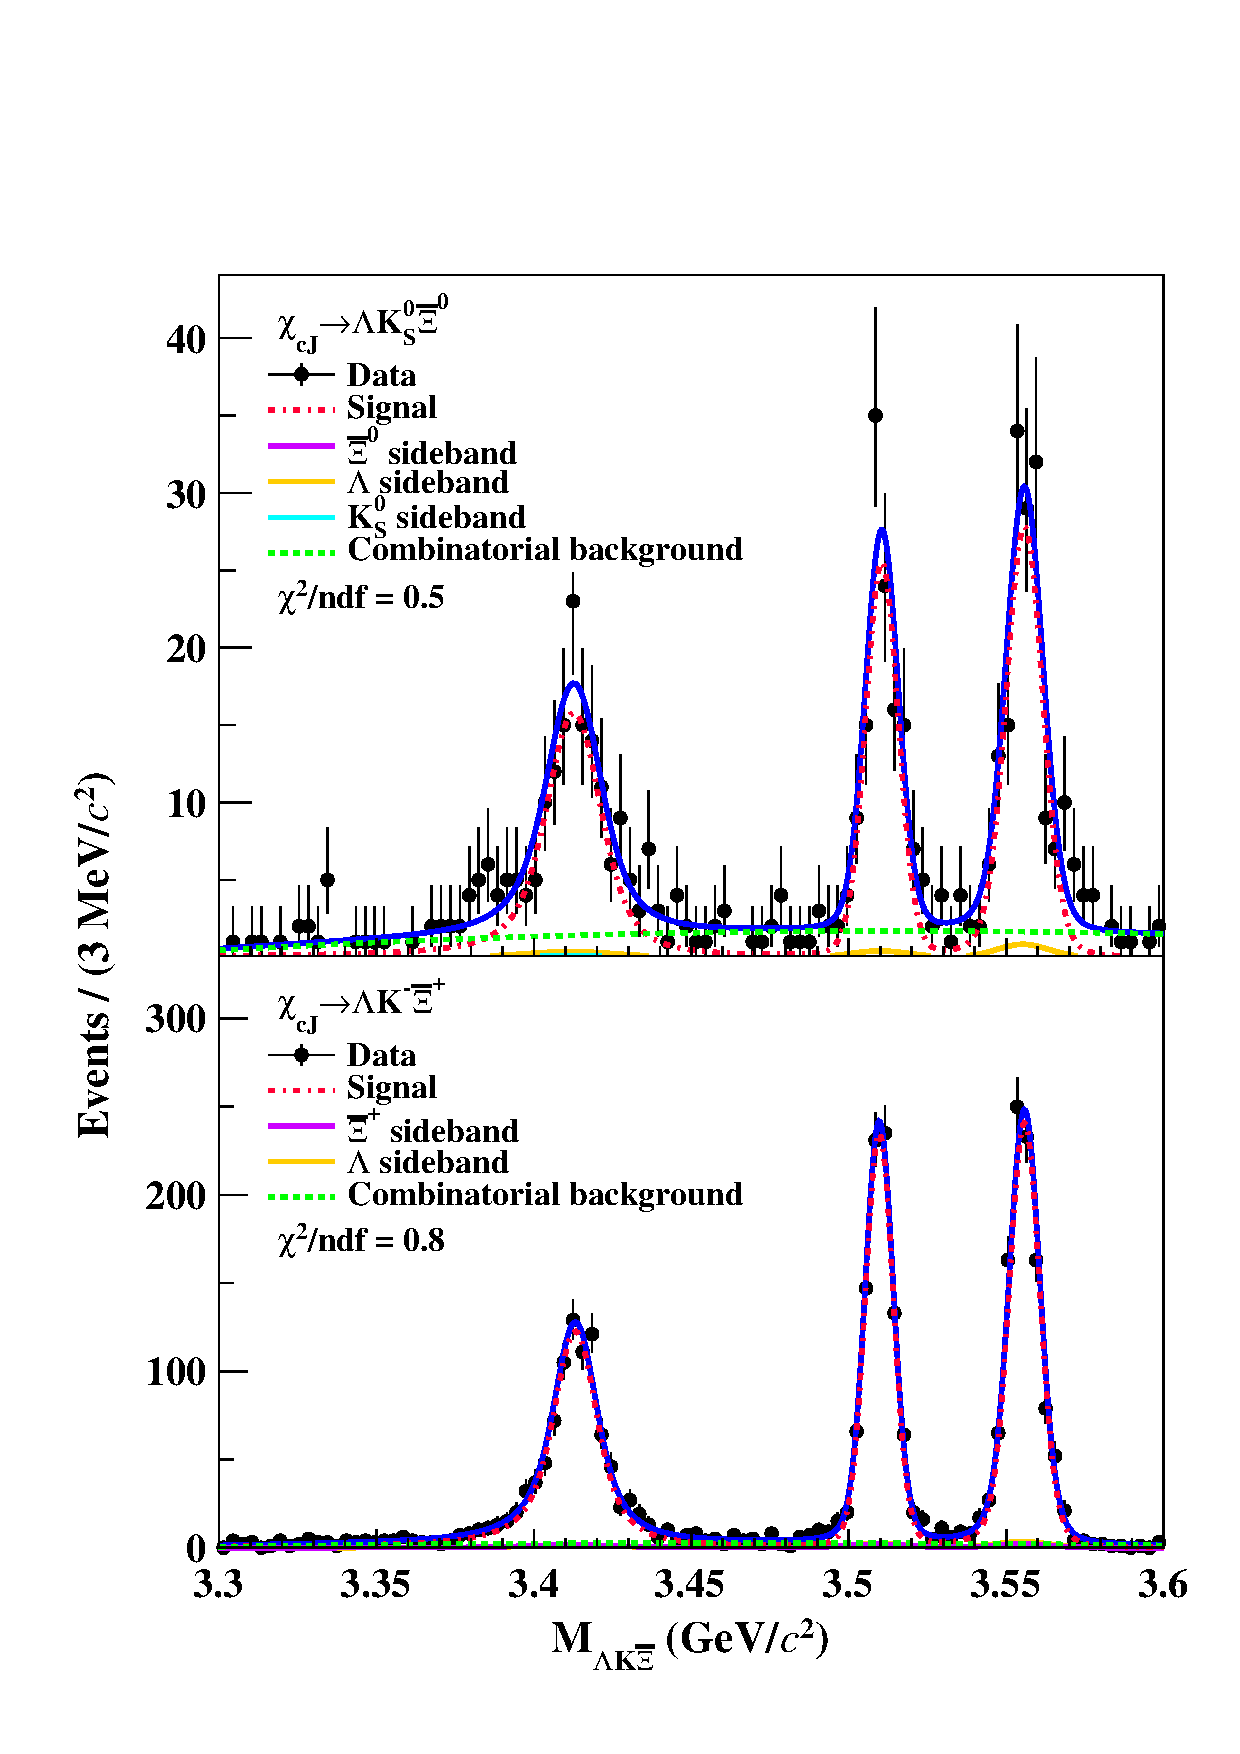
\includegraphics[width=8cm]{LambdaXiK_fit.pdf}
	\caption{The simultaneous fits to the $M_{\Lambda K \bar \Xi}$ distributions in the $\bar \Xi$, $\Lambda$, (and $K^0_S$) signal and sideband regions for (top) $\chi_{cJ}\to \Lambda K^0_S \bar \Xi^0$ and (bottom) $\chi_{cJ}\to \Lambda K^- \bar \Xi^+$. The black dots with error bars are data. The blue solid curves are the fit results. The red dashed curves are the fitted signals. The purple solid, orange solid, zerue solid curves denote the peaking background contributions, respectively, constrained by the $\bar \Xi$, $\Lambda$, and $K^0_S$ sideband events in data; and the green dashed curves are the fitted combinatorial background shapes.}
	\label{tab:LambdaKXi}
\end{figure}
		
Figure~\ref{fig:compare_LXiKS} and \ref{fig:compare_LXiK} show the comparisons of the two-body invariant-mass distributions for the $\chi_{cJ} \to \Lambda K^0_S\bar{\Xi}^0$ and $\chi_{cJ} \to \Lambda K^-\bar{\Xi}^+$ decays in data and mixed signal MC samples. Good data-MC consistencies ensure the reliability of the detection efficiencies.
The obtained detection efficiencies for $\chi_{cJ} \to \Lambda K^0_S\bar \Xi^0$ and  $\chi_{cJ} \to \Lambda K^-\bar \Xi^+$ are shown in Table \ref{tab:BFs_neutral} and Table \ref{tab:BFs_charged}.

\begin{figure*}[htbp]
	\centering
	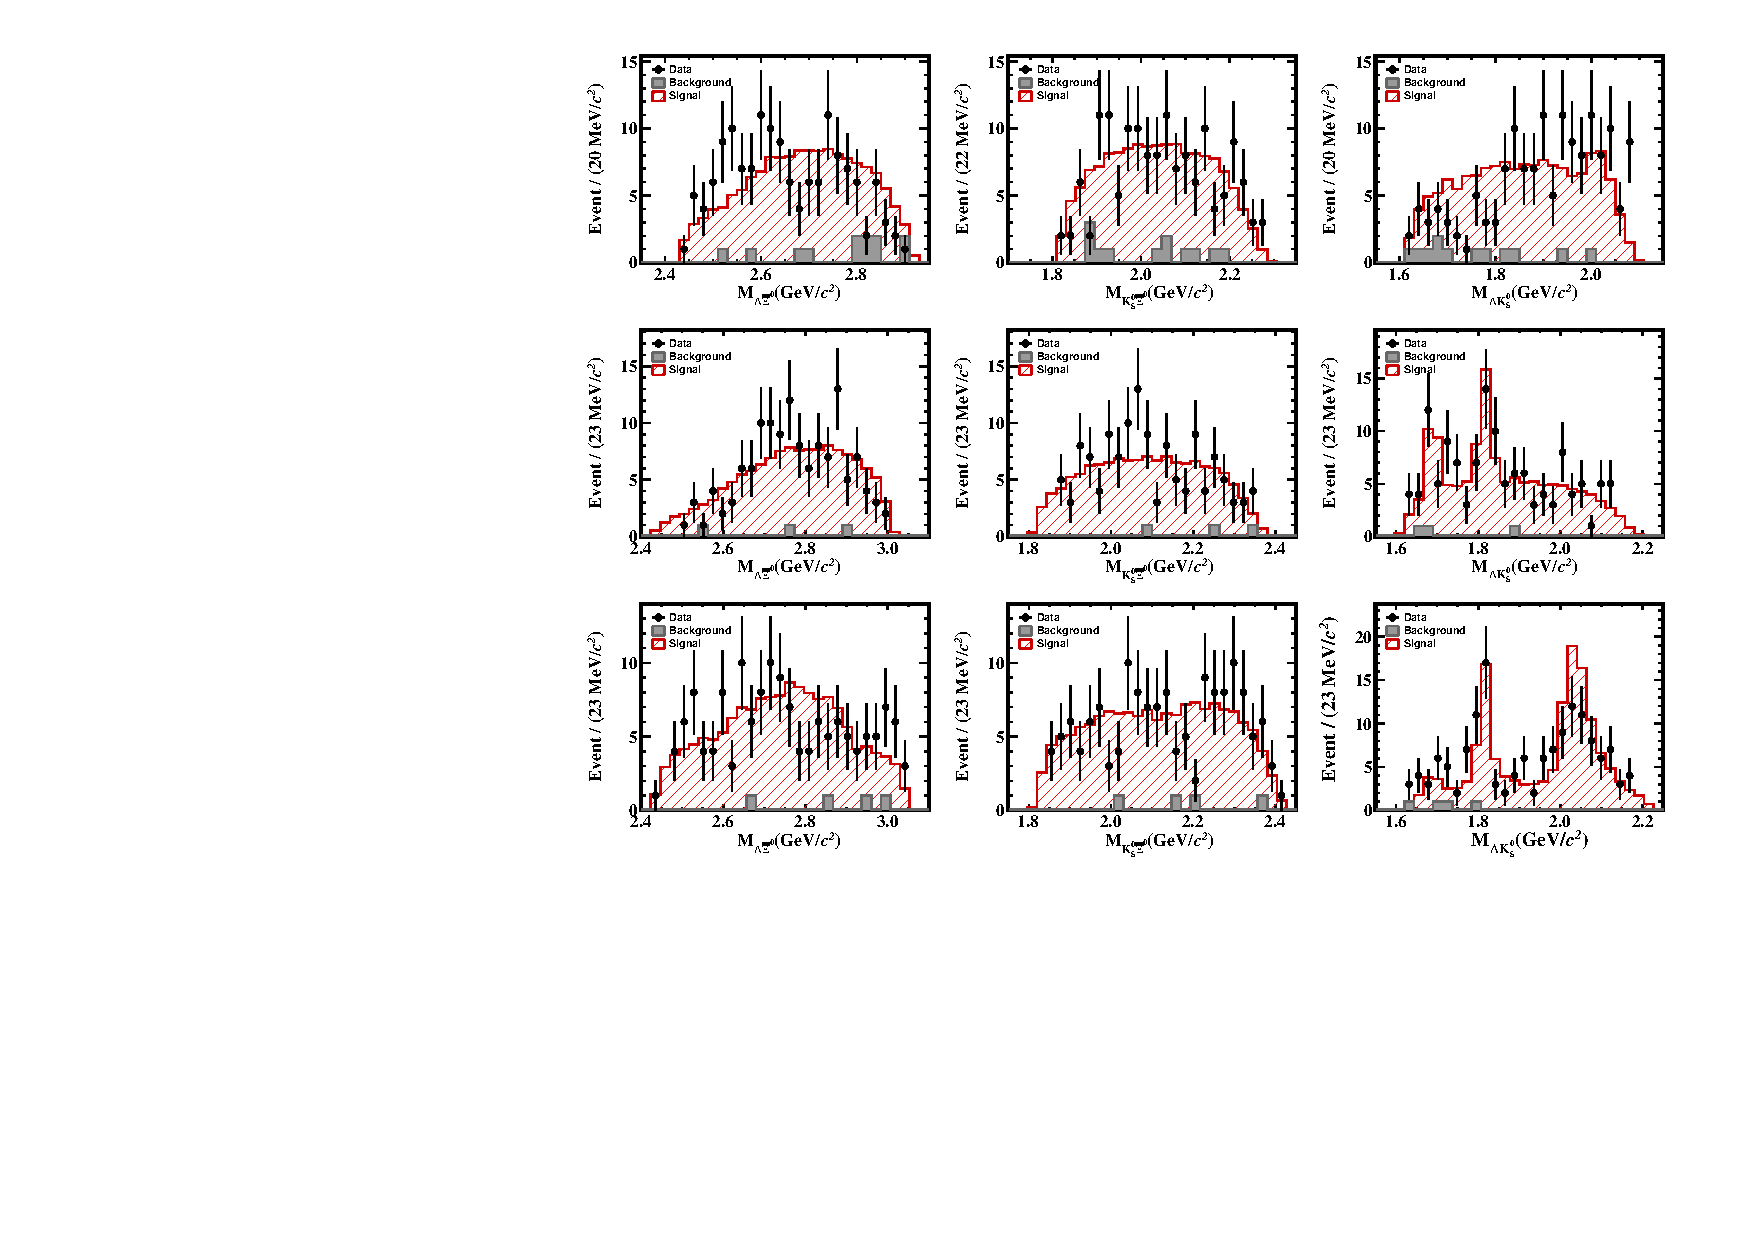
\includegraphics[width=13cm]{compare9_37_cJ.pdf}	
	\caption{Comparisons of $M_{\Lambda \bar \Xi^0}$, $M_{K^0_S \bar \Xi^0}$, and $M_{\Lambda K^0_S}$ of the accepted candidates for $\chi_{cJ} \to \Lambda K^0_S \bar{\Xi}^0$. The black dots with error bars represent data, the histograms filled with red lines denote the mixed signal MC samples, and the grey histograms show the background contributions from the inclusive MC sample. Events have been required to be within the (top) $\chi_{c0}$, (middle) $\chi_{c1}$, and (down) $\chi_{c2}$, 
	 mass regions defined by $M_{\Lambda K^0_S \bar{\Xi}^0} \in [3.400, 3.430]$, $[3.501, 3.521]$, and $[3.546, 3.566]$ GeV/$c^2$, respectively.}
	\label{fig:compare_LXiKS}
\end{figure*}

\begin{figure*}[htbp]
	\centering
	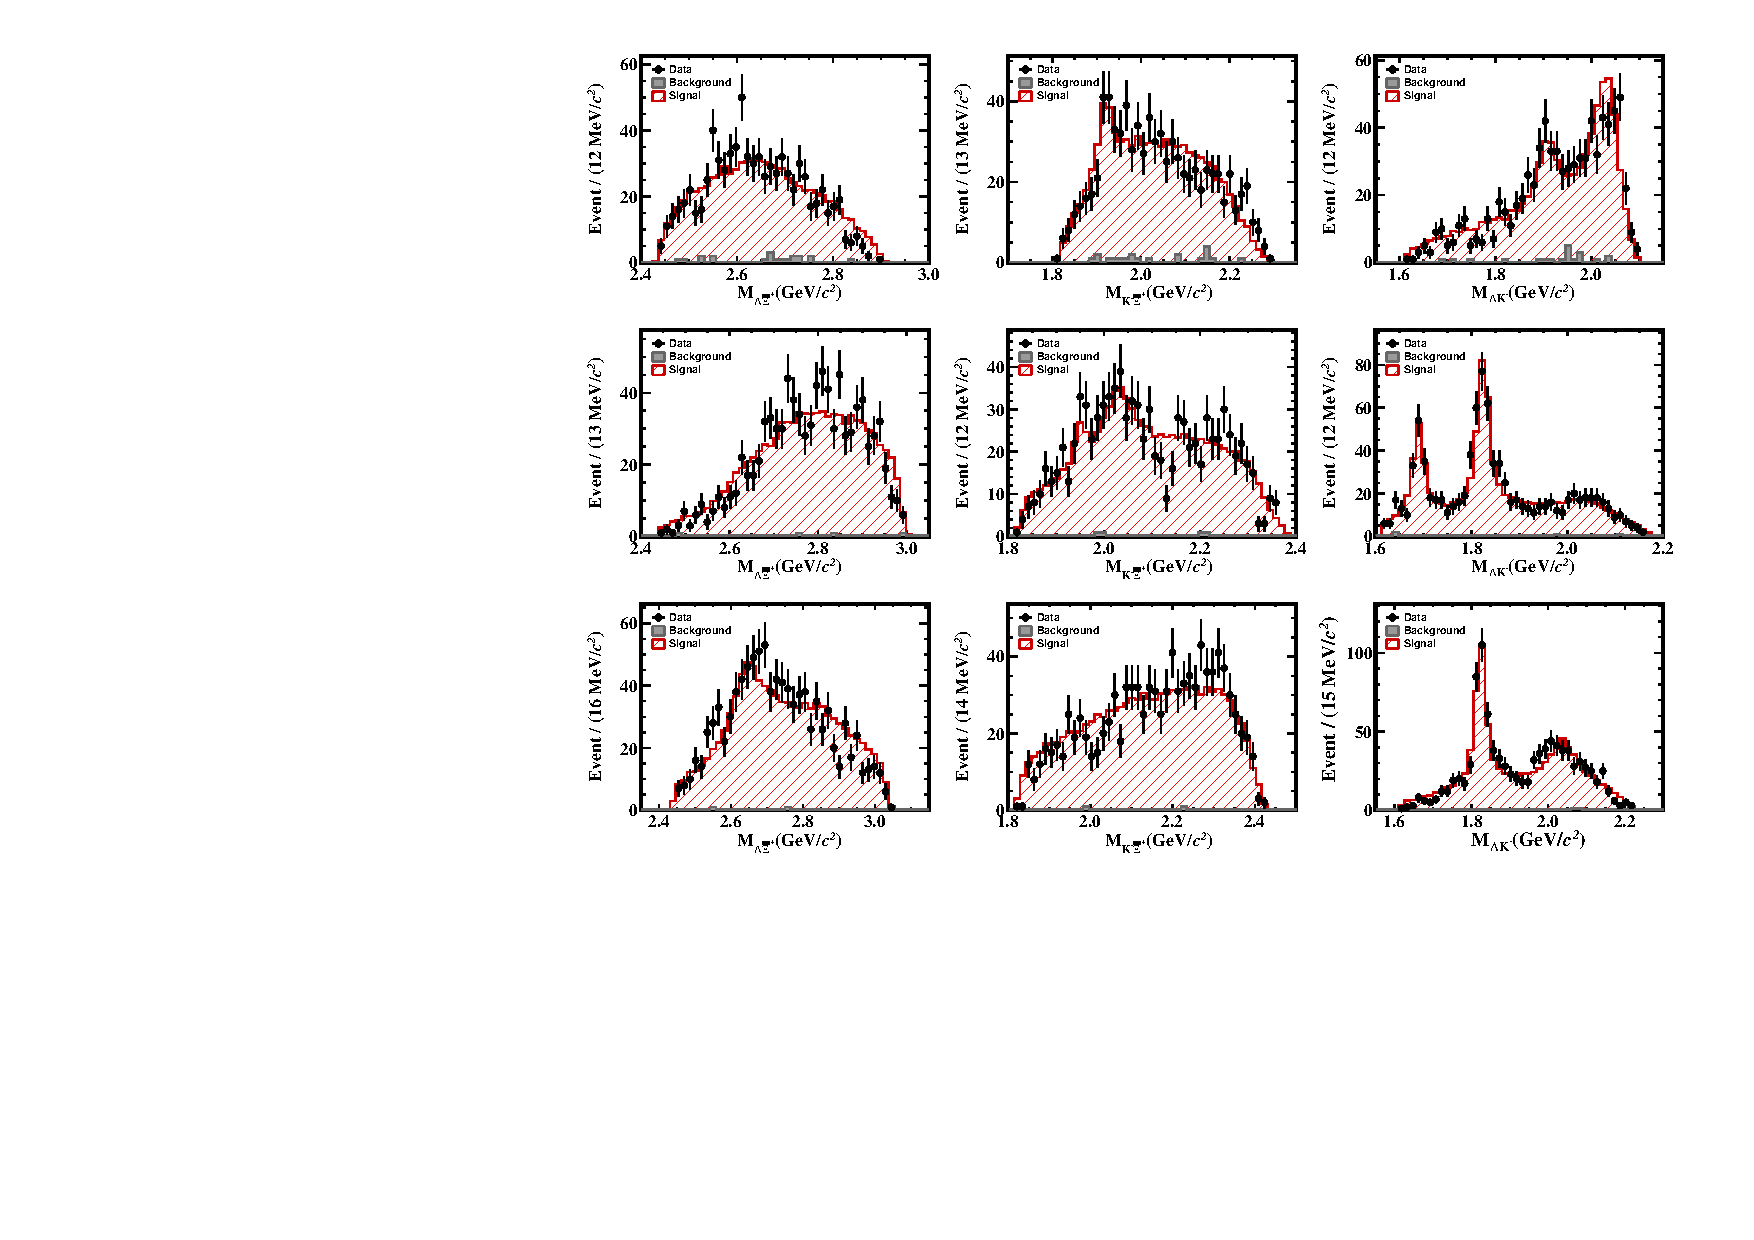
\includegraphics[width=13cm]{compare9_36_cJ.pdf}	
	\caption{Comparisons of $M_{\Lambda \bar \Xi^+}$, $M_{K^- \bar \Xi^+}$, and $M_{\Lambda K^-}$ of the accepted candidates for $\chi_{cJ} \to \Lambda K^- \bar{\Xi}^+$. The black dots with error bars represent data, the histograms filled with red lines denote the mixed signal MC samples, and the grey histograms show the background contributions from the inclusive MC sample. Events have been required to be within the (top) $\chi_{c0}$, (middle) $\chi_{c1}$, and (down) $\chi_{c2}$, mass regions defined by $M_{\Lambda K^- \bar{\Xi}^+} \in [3.400, 3.430]$, $[3.501, 3.521]$, and $[3.546, 3.566]$ GeV/$c^2$, respectively.}
	\label{fig:compare_LXiK}
\end{figure*}

The product of branching fractions are calculated as
\begin{linenomath*}
	\begin{equation}
		{\mathcal B}(\psi(3686)\to \gamma\chi_{cJ}) \cdot \mathcal{B}(\chi_{cJ}\to \Lambda K \bar \Xi)
		=\frac{N^{\rm obs}_{\chi_{cJ}}}{N_{\psi(3686)}\cdot\epsilon \cdot \mathcal B_{\rm sub}},
	\end{equation}
\end{linenomath*}
where $\mathcal{B}(\chi_{cJ}\to \Lambda K \bar \Xi)$ is the branching fractions of $\chi_{cJ}$ decaying to the final state, $N_{\psi(3686)}$ is the total number of $\psi(3686)$ events in data, and $\epsilon$ is the detection efficiency. The variable $\mathcal B_{\rm sub}$ is
$\mathcal B(K^0_S \to \pi^+ \pi^-) \cdot \mathcal B^2(\Lambda  \to p \pi^-) \cdot \mathcal B(\bar\Xi^0  \to\bar \Lambda \pi^0)
\cdot \mathcal B(\pi^0 \to \gamma\gamma)$ for the calculation of the branching fractions of  $\chi_{cJ} \to \Lambda K^0_S \bar \Xi^0$, and
$\mathcal B^2(\Lambda  \to p \pi^-) \cdot \mathcal B(\bar\Xi^+  \to\bar \Lambda \pi^-)$
for $\chi_{cJ} \to \Lambda K^-\bar \Xi^+$.
Combining the branching fractions of $\psi(3686)\to\gamma\chi_{cJ}$ quoted from the PDG~\cite{ref::pdg2024}, 
the branching fractions of the $\chi_{cJ} \to \Lambda K \bar \Xi$ decays are determined. All the obtained results for $\chi_{cJ}\to \Lambda K^0_S \bar \Xi^0$ and $\chi_{cJ}\to \Lambda K^- \bar \Xi^+$ are summarized in Table \ref{tab:BFs_neutral} and Table \ref{tab:BFs_charged}.

\begin{table*}[htbp]
	\caption{Quantities used for  the branching fractions calculations for $\chi_{cJ} \to \Lambda K^0_S\bar \Xi^0$, where the first uncertainties are statistical and the second uncertainties are systematic.}
	\centering
	%		\resizebox{1\textwidth}{!}{
		\begin{tabular}{lccc}
			\hline\hline
			& $ \chi_{c0}\to \Lambda K^0_S\bar{\Xi}^0$ & $ \chi_{c1}\to \Lambda K^0_S\bar{\Xi}^0$ & $ \chi_{c2}\to \Lambda K^0_S\bar{\Xi}^0 $ \\ 
			\hline   
			$N_{\rm sig}$ & $139\pm15$ & $113\pm12$ & $144\pm14$ \\ 
			$\epsilon~(\%)$ & $1.637\pm0.013$ & $2.015\pm0.014$ & $1.724\pm0.013$ \\
			$\mathcal{B}(\psi(3686)\to \gamma \chi_{cJ})\cdot\mathcal{B}(\chi_{cJ}\to \Lambda K^0_S\bar \Xi^0)~(10^{-5})$ & $1.12\pm0.12\pm0.13$ & $0.74\pm0.08\pm0.06$ & $1.10\pm0.11\pm0.13$ \\ 
			$\mathcal{B}(\chi_{cJ}\to \Lambda K^0_S\bar \Xi^0)~(10^{-4})$  & $1.14\pm0.13\pm0.13$ & $0.76\pm0.08\pm0.07$ & $1.18\pm0.11\pm0.14$ \\ \hline 
			\hline
		\end{tabular}
		\label{tab:BFs_neutral}
	\end{table*}
	
	\begin{table*}[htbp]
		\caption{Quantities used for  the branching fractions calculations for $\chi_{cJ} \to \Lambda K^-\bar \Xi^+$, where the first uncertainties are statistical and the second uncertainties are systematic.}
		\centering
		%		\resizebox{1\textwidth}{!}{
			\begin{tabular}{lccc}
				\hline\hline
				& $ \chi_{c0} \to \Lambda K^-\bar{\Xi}^+$ & $ \chi_{c1} \to \Lambda K^-\bar{\Xi}^+$ & $ \chi_{c2} \to \Lambda K^-\bar{\Xi}^+ $ \\ 
				\hline 
				$N_{\rm sig}$ & $909\pm35$ & $896\pm32$ & $1054\pm35$ \\ 
				$\epsilon~(\%)$ & $4.281\pm0.021$ & $5.870\pm0.024$ & $5.033\pm0.022$ \\ 
				$\mathcal{B}(\psi(3686)\to \gamma \chi_{cJ})\cdot\mathcal{B}(\chi_{cJ}\to \Lambda K^-\bar \Xi^+)~(10^{-5})$ & $1.91\pm0.07\pm0.16$ & $1.37\pm0.05\pm0.11$ & $1.88\pm0.06\pm0.15$ \\                    
				$\mathcal{B}(\chi_{cJ}\to \Lambda K^-\bar \Xi^+)~(10^{-4})$& $1.95\pm0.08\pm0.17$ & $1.41\pm0.05\pm0.11$ & $2.01\pm0.07\pm0.16$ \\ \hline
				\hline
			\end{tabular}
			\label{tab:BFs_charged}
		\end{table*}
		
\section{SYSTEMATIC UNCERTAINTY}

The systematic uncertainties in the branching fraction measurements arise from various sources, as summarized in Table~\ref{tab:systematic}. These uncertainties are estimated and discussed below.

The total number of $\psi(3686)$ events in data is measured to be $N_{\psi(3686)}=(2712.4\pm14.3)\times10^6$ with the inclusive hadronic events as described in Ref.~\cite{ref::psip-num-inc}. The uncertainty of $N_{\rm \psi(3686)}$ is 0.5\%.

The systematic uncertainties of the tracking or PID for $K^{\pm}$ and $p(\bar{p})$ are estimated with the control samples of $J/\psi\to K^{+}K^{-}\pi^0$ and $J/\psi \to p\bar p \pi^+\pi^-$. They are assigned as 1.0\% for tracking or PID per track~\cite{ref::tracking}.

The systematic uncertainty of the $K^0_S$ reconstruction, including tracking, $K^0_S$ mass window, vertex fit, and secondary vertex fit, is estimated using the control sample of $J/\psi \rightarrow K^{*\pm} ¯\bar{K}^\mp$ and $J/\psi \rightarrow \phi K^{*\pm} ¯\bar{K}^\mp$. The systematic uncertainty of the $K^0_S$ reconstruction is assigned to be 1.5\%~\cite{ref::kso}.

The systematic uncertainty of $\Lambda$ reconstruction, including the tracking of the $p\pi^-$ pair, decay length cut, mass window cut, vertex fit and secondary vertex fit, are studied by using the control sample of $J/\psi\to pK^-\bar \Lambda$ and $J/\psi\to\Lambda\bar \Lambda$. The obtained efficiencies in the 2D intervals are weighted by the 2D distributions of various momentum and $\cos\theta$ to match our signal MC events, according to Ref.~\cite{ref::Lambda}. The differences of the re-weighted efficiencies between data and MC simulation are assigned as the systematic uncertainties, which are 2.9\%, 1.6\%, 3.5\% for $\chi_{c0,1,2}\to \Lambda K^0_S\bar \Xi^0$; and
2.9\%, 2.5\%, and 2.5\% for $\chi_{c0,1,2}\to \Lambda K^-\bar \Xi^+$,~respectively.

The systematic uncertainty of $\bar\Xi^+$ reconstruction is estimated to be $5.1\%$, including the tracking and PID of the $\bar{\Lambda}\pi^+$ pair, $\Lambda$ reconstruction, decay length cut, mass window cut, vertex fit and secondary vertex fit, by studying the control sample of $\psi(3686)\to\Xi^-\bar{\Xi}^+$ as in Ref.~\cite{ref::Xi}. The systematic uncertainty of $\bar\Xi^0$ reconstruction is estimated to be $4.5\%$, including the tracking and PID of the $\bar{\Lambda}\pi^0$ pair, $\pi^0$ reconstruction, decay length cut, and mass window cut, by studying the control sample of $\psi(3686)\to\Xi^0\bar{\Xi}^0$.

The systematic uncertainty of photon or $\pi^0$ reconstruction is assigned as  1.0\% per photon based on the control sample of $J/\psi\to\pi^+\pi^-\pi^0$~\cite{ref::gamma-recon}.

To estimate the systematic uncertainties associated with variations in the sub-resonant fractions of the MC model for the $\chi_{cJ}\to \Lambda K\bar \Xi$ decays, we compare our nominal signal efficiencies with those determined from the mixed signal MC events after varying the relative fractions of the sub-resonant decays, such as 
$\chi_{cJ}\to \Xi(1690)\bar{\Xi}$, $\chi_{cJ}\to \Xi(1820)\bar{\Xi}$, and $\chi_{cJ}\to \Xi(2030)\bar{\Xi}$, by $\pm 1\sigma$. The changes of the signal efficiencies, 3.2\%, 0.2\%, and 0.9\%, are taken as the systematic uncertainties for \chic{0}, \chic{1}, and \chic{2} decays to $\Lambda K^0_S\bar \Xi^0$, respectively. The relative changes in the signal efficiencies, 3.5\%, 0.1\%, and 0.9\%, are assigned as the corresponding systematic uncertainties for \chic{0}, \chic{1}, and \chic{2} decays to $\Lambda K^-\bar \Xi^+$, respectively.

The systematic uncertainties associated with the fits to the $M_{\Lambda K \bar{\Xi}}$ distributions are evaluated by considering several sources. The uncertainty due to the signal shape is estimated by comparing the fitted signal yields obtained with alternative fits varying the width within $\pm1\sigma$. The uncertainty related to the background shape is evaluated by varying the order of the polynomial used to describe the background in the fit. The uncertainty associated with the fitting range is estimated by repeating the fits with alternative fit ranges for the $M_{\Lambda K \bar{\Xi}}$ spectra, from [3.28,3.58] to [3.35,3.65]~GeV/$c^2$. In addition, the uncertainty from the normalization between the signal and sideband regions is evaluated by varying the corresponding scaling factors to the ratio of the event yields between the signal and sideband regions determined from fits to the $M_{\Lambda\pi^0}$, $M_{\Lambda\pi^-}$, $M_{p\pi^-}$, and $M_{\pi^+\pi^-}$ distributions in data. The systematic uncertainty due to peaking backgrounds from $\chi_{cJ}\to\Sigma^0K\bar{\Xi}$ is estimated by including the MC-simulated peaking background component as an additional probability density function in the fit, with the yields and relative fractions among the $\chi_{cJ}$ states fixed according to expectations. For each source, the difference between the re-fitted and nominal signal yields is taken as the corresponding systematic uncertainty, and the total systematic uncertainty associated with the fit is obtained by adding all contributions in quadrature.

The systematic uncertainties due to the fit bias are estimated by performing input-output checks based on the inclusive MC sample.
The differences between the measured and input branching fractions are taken as the systematic uncertainties,
which are~3.0\%, 3.0\%, and 1.0\% for  $\chi_{c1}\to \Lambda K^0_S\bar \Xi^0$, $\chi_{c2}\to \Lambda K^0_S\bar \Xi^0$, and $\chi_{c2}\to \Lambda K^-\bar \Xi^+$,~which are negligible for other decays. 

The systematic uncertainty from the 4C kinematic fit is estimated by comparing the signal efficiencies before and after applying a helix parameter correction.
The correction factors are obtained from Ref.~\cite{ref::helixp}.
The changes in the signal efficiencies are assigned as the systematic uncertainties, which are 3.2\%, 1.1\%, and 2.9\% for $\chi_{c0,1,2}\to \Lambda K^0_S\bar \Xi^0$; and 1.9\%, 0.2\%, and 0.3\% for $\chi_{c0,1,2}\to \Lambda K^-\bar \Xi^+$,~respectively.

The systematic uncertainties due to the limited statistics of the mixed signal MC samples
are 0.7\%, 0.6\%, and 0.7\% for  $\chi_{c0,1,2}\to  \Lambda K^0_S\bar \Xi^0$,
and 0.500\%, 0.4\%, and 0.4\% for $\chi_{c0,1,2}\to \Lambda K^-\bar \Xi^+$,~respectively.

The uncertainties from the branching fractions quoted from the PDG~\cite{ref::pdg2024} are 2.3\%, 2.8\%, and 2.4\% for $\psi(3686)\to \gamma\chi_{c0,1,2}$,
0.07\% for $\mathcal{B}(K^{0}_{S} \to \pi^+ \pi^-)$, 0.800\% for $\mathcal{B}(\Lambda \to p \pi^-)$, 0.010\% for $\mathcal{B}(\bar{\Xi}^0 \to \Lambda\pi^0)$, 0.03\% for $\mathcal{B}(\bar{\Xi}^- \to \Lambda \pi^-)$, and 0.03\% for $\mathcal{B}(\pi^0 \to \gamma \gamma)$,  

For each signal decay, the total systematic uncertainty is obtained by adding all individual systematic uncertainties in quadrature.

\begin{table}[htbp]
	\centering
	\caption{Relative systematic uncertainties (in \%) in the measurements of the branching fractions of $\chi_{cJ} \to \Lambda K^0_S \bar \Xi^0$ and $\chi_{cJ} \to \Lambda K^- \bar \Xi^+$.}
	\begin{tabular}{lcccccc}
		\hline\hline
		&\multicolumn{3}{c}{$\Lambda K^0_S \bar \Xi^0$}&\multicolumn{3}{c}{$\Lambda K^- \bar \Xi^+$} \\ \hline
		Source & $\chi_{c0}$ & $\chi_{c1}$ & $\chi_{c2}$ & $\chi_{c0}$ & $\chi_{c1}$ & $\chi_{c2}$ \\ \hline
		$N_{\psi(3686)}$ & 0.5 & 0.5 & 0.5 & 0.5 & 0.5 & 0.5\\
		$K^-$ tracking & ... & ... & ... & 1.0 & 1.0 & 1.0\\
		$K^-$ or $p$ PID & 2.0 & 2.0 & 2.0 & 3.0 & 3.0 & 3.0 \\
		$K_{S}^{0}$ reconstruction & 1.5 & 1.5 & 1.5 & ... & ... & ...\\
		$\Lambda$ reconstruction & 2.90 & 1.60 & 3.5 & 2.9 & 2.5 & 2.5\\
		$\bar\Xi^+$ reconstruction & ... & ... & ... & 5.1 & 5.1 & 5.1 \\
		$\bar\Xi^0$ reconstruction & 4.5 & 4.5 & 4.5 & ... & ... & ... \\
		$\gamma$ reconstruction & 1.0 & 1.0 & 1.0 & 1.0 & 1.0 & 1.0 \\
		4C kinematic fit & 3.2 & 1.1 & 2.9 & 1.9 & 0.2  & 0.3\\
		$M_{\Lambda K \bar \Xi}$ fit  & 8.6 & 5.9 & 8.7 & 2.7 & 2.5 & 4.1\\
		Fitting bias & 0.0 & 3.0 & 3.0 & 0.0 & 0.0  & 1.0\\
		$\mathcal B(K_{S}^{0} \to \pi^{+} \pi^{-})$ & 0.1 & 0.1 & 0.1 & ... & ... & ...\\
		$\mathcal B(\pi^0 \to \gamma\gamma )$ & 0.0 & 0.0 & 0.0 & ... & ... & ...\\
		$\mathcal B(\psi(3686)\to \gamma \chi_{cJ})$ & 2.3 & 2.8 & 2.4 & 2.3 & 2.8 & 2.4 \\
		$\mathcal B(\Lambda \to p\pi^-)$ & 1.6 & 1.6 & 1.6  & 1.6 & 1.6 & 1.6 \\
		$\mathcal B(\bar \Xi^0\to \bar \Lambda\pi^0)$ & 0.0 & 0.0 & 0.0 & ... & ... & ...\\
		$\mathcal B(\bar \Xi^+\to \bar \Lambda\pi^+)$ & ... & ... & ... & 0.0 & 0.0 & 0.0 \\
		MC statistics & 0.7 & 0.6 & 0.7 & 0.5 & 0.4 & 0.4 \\
		MC generator  & 3.2 & 0.2 & 0.9 & 3.5 & 0.1 & 0.9\\
		Total~(without $\mathcal B(\psi^{'} \to \chi_{cJ})$)  & 11.7 & 8.2 & 11.3 & 8.2 & 7.5 & 7.7\\
		Total~(with $\mathcal B(\psi^{'} \to \chi_{cJ})$)  & 11.5 & 8.7 & 11.6 & 8.5 & 8.0 & 8.0\\
		\hline\hline
	\end{tabular}
	\label{tab:systematic}
\end{table}


\section{Summary}

Using $(2712.4\pm14.3)\times10^6$ $\psi(3686)$ events collected with the BESIII detector operating at the BEPCII collider,
the hadronic decays of $\chi_{cJ}\to \Lambda K^0_S\bar \Xi^0$ are observed for the first time, with  significances greater than $10\sigma$,
the decays of $\chi_{cJ}\to \Lambda K^-\bar \Xi^+$ are measured with improved precision.
Their decay branching fractions are determined to be
$\mathcal{B}(\chi_{c0}\to \Lambda K^0_S\bar \Xi^0)=(1.14\pm0.13\pm0.13)\times10^{-4}$,
$\mathcal{B}(\chi_{c1}\to \Lambda K^0_S\bar \Xi^0)=(7.6\pm0.8\pm0.7)\times10^{-5}$,
$\mathcal{B}(\chi_{c2}\to \Lambda K^0_S\bar \Xi^0)=(1.18\pm0.11\pm0.14)\times10^{-4}$,
$\mathcal{B}(\chi_{c0}\to \Lambda K^-\bar \Xi^+)=(1.95\pm0.08\pm0.17)\times10^{-4}$,
$\mathcal{B}(\chi_{c1}\to \Lambda K^-\bar \Xi^+)=(1.41\pm0.05\pm0.11)\times10^{-4}$, and 
$\mathcal{B}(\chi_{c2}\to \Lambda K^-\bar \Xi^+)=(2.01\pm0.07\pm0.16)\times10^{-4}$.
These measurements will be helpful for understanding $\chi_{cJ}$ decay mechanisms. 
The ratios of the branching fractions, ${\mathcal B}(\chi_{cJ}\to\Lambda K^0_S\bar{\Xi}^0)/{\mathcal B}(\chi_{cJ}\to\Lambda K^-\bar{\Xi}^+)$, are calculated to be $0.59\pm0.07\pm0.06$, $0.54\pm0.06\pm0.06$, and $0.59\pm0.06\pm0.06$ for $\chi_{c0}$, $\chi_{c1}$, and $\chi_{c2}$ decays. These results support that isospin symmetry holds in these decays. In determining these ratios, the systematic uncertainties associated with the total number of $\psi(3686)$ events, the photon radiated from $\psi(3686)$, and the external branching fractions $\mathcal B(\psi(3686)\to \gamma \chi_{cJ})$ and $\mathcal B(\Lambda \to p\pi^-)$, cancel in the ratio measurement. The measured ratios are consistent with the theoretical expectation of ${\mathcal B}(\chi_{cJ}\to\Lambda K^0_S\bar{\Xi}^0)/{\mathcal B}(\chi_{cJ}\to\Lambda K^-\bar{\Xi}^+)=0.5$ within uncertainties. In addition, we have also examined the mass spectra of $\Lambda \bar \Xi$, and no threshold enhancements are found under the current statistics.

\section{Acknowledgement}

The BESIII Collaboration thanks the staff of BEPCII {\hypersetup{urlcolor=black}\href{https://cstr.cn/31109.02.BEPC}{(https://cstr.cn/31109.02.BEPC)}} and the IHEP computing center for their strong support. This work is supported in part by National Key R\&D Program of China under Contracts Nos. 2020YFA0406300, 2020YFA0406400, 2023YFA1606000; National Natural Science Foundation of China (NSFC) under Contracts Nos. 12035009, 11875170, 11635010, 11735014, 11935015, 11935016, 11935018, 12025502, 12035013, 12061131003, 12192260, 12192261, 12192262, 12192263, 12192264, 12192265, 12221005, 12225509, 12235017, 12361141819; the Chinese Academy of Sciences (CAS) Large-Scale Scientific Facility Program; the CAS Center for Excellence in Particle Physics (CCEPP); Joint Large-Scale Scientific Facility Funds of the NSFC and CAS under Contract No. U1832207; 100 Talents Program of CAS; The Institute of Nuclear and Particle Physics (INPAC) and Shanghai Key Laboratory for Particle Physics and Cosmology; German Research Foundation DFG under Contracts Nos. FOR5327, GRK 2149; Istituto Nazionale di Fisica Nucleare, Italy; Knut and Alice Wallenberg Foundation under Contracts Nos. 2021.0174, 2021.0299; Ministry of Development of Turkey under Contract No. DPT2006K-120470; National Research Foundation of Korea under Contract No. NRF-2022R1A2C1092335; National Science and Technology fund of Mongolia; National Science Research and Innovation Fund (NSRF) via the Program Management Unit for Human Resources \& Institutional Development, Research and Innovation of Thailand under Contracts Nos. B16F640076, B50G670107; Polish National Science Centre under Contract No. 2019/35/O/ST2/02907; Swedish Research Council under Contract No. 2019.04595; The Swedish Foundation for International Cooperation in Research and Higher Education under Contract No. CH2018-7756; U. S. Department of Energy under Contract No. DE-FG02-05ER41374.









\begin{thebibliography}{99}
\bibitem{ref::eetochic1} S. Spataro {\it et al.} (BESIII Collaboration), \href{https://doi.org/10.22323/1.476.0494}{PoS (ICHEP2024) 494 (2024)}
\bibitem{ref::pdg2024} S. Navas {\it et al.} (Particle Data Group), \href{https://journals.aps.org/prd/pdf/10.1103/PhysRevD.110.030001}{Phys. Rev. D {\bf 110}, 030001 (2024).}
\bibitem{ref::pppipi} J. Z. Bai {\it et al.} (BES Collaboration), \href{https://doi.org/10.1103/PhysRevD.60.072001}{Phys. Rev. D {\bf 60}, 072001 (1999).}
\bibitem{ref::pppi0pi0}Q. He {\it et al.} (CLEO Collaboration), \href{https://doi.org/10.1103/PhysRevD.78.092004}{Phys. Rev. D {\bf 78}, 092004 (2008).}
\bibitem{ref::ppkk}M. Ablikim {\it et al.} (BESIII Collaboration), \href{https://doi.org/10.1103/PhysRevD.83.112009}{Phys. Rev. D {\bf 83}, 112009 (2011).}
\bibitem{ref::lambdalambdabar}M. Ablikim {\it et al.} (BESIII Collaboration), \href{https://doi.org/10.1103/PhysRevD.103.112004}{Phys. Rev. D {\bf 103}, 112004 (2021).}
\bibitem{ref::sigmasigmabar}M. Ablikim {\it et al.} (BESIII Collaboration), \href{https://doi.org/10.1103/PhysRevD.97.052011}{Phys. Rev. D {\bf 97}, 052001 (2018).}
\bibitem{ref::oct1}J. Bolz, P. Kroll, and G. A. Schuler, \href{http://dx.doi.org/10.1016/S0370-2693(96)01515-8}{Phys. Lett. B {\bf 292}, 192 (1997).}
\bibitem{ref::oct2}S. M. Wong {\it et al.}, \href{http://dx.doi.org/10.1007/s100520000376}{Eur. Phys. J. C {\bf 14}, 643 (2000).}
\bibitem{ref::ppbar1} J. Z. Bai {\it et al.} (BES Collaboration), \href{https://doi.org/10.1103/PhysRevLett.91.022001}{Phys. Rev. Lett. {\bf 91}, 022001 (2003).}
\bibitem{ref::ppbar2} M. Ablikim {\it et al.} (BESIII Collaboration), \href{https://doi.org/10.1103/PhysRevLett.108.112003}{Phys. Rev. Lett. {\bf 108}, 112003 (2012).}
\bibitem{ref::LXiK} M. Ablikim {\it et al.} (BESIII Collaboration), \href{https://journals.aps.org/prd/abstract/10.1103/PhysRevD.91.092006}{Phys. Rev. D. {\bf 91}, 092006 (2015).}
\bibitem{ref::psip-num-inc} M. Ablikim {\it et al.} (BESIII Collaboration),
\href{http://arxiv.org/abs/2403.06766}{arXiv 2403 06776}
\bibitem{ref::detector} M. Ablikim {\it et al.} (BESIII Collaboration), \href{https://www.sciencedirect.com/science/article/pii/S0168900209023870}{Nucl. Instrum. Methods Phys. Res., A {\bf614}, 345 (2010).}	
\bibitem{ref::collider} C.~H.~Yu {\it et al.}, \href{https://accelconf.web.cern.ch/ipac2016/doi/JACoW-IPAC2016-TUYA01.html}{Proceeding of IPAC2016, Busan, Korea, 2016}
\bibitem{Tof1} X.~Li {\it et al.}, \href{https://link.springer.com/article/10.1007/s41605-017-0014-2} {Radiat. Detect. Technol. Methods {\bf 1}, 13 (2017).}

\bibitem{Tof2} Y.~X.~Guo {\it et al.}, \href{https://link.springer.com/article/10.1007/s41605-017-0012-4} {Radiat. Detect. Technol. Methods {\bf 1}, 15 (2017).}

\bibitem{Tof3} P.~Cao {\it et al.}, \href{https://www.sciencedirect.com/science/article/pii/S0168900219314068} {Nucl. Instrum. Meth. A {\bf 953}, 163053 (2020).}

\bibitem{Geant4} S.~Agostinelli \textit{et al.} ({\sc geant4} Collaboration), \href{https://www.sciencedirect.com/science/article/pii/S0168900203013688?via\%3Dihub}{Nucl. Instrum. Methods Phys. Res. {A \bf506}, 250 (2003).}
\bibitem{Jadach01} S.~Jadach, B.~F.~L.~Ward~and Z.~Was, \href{https://journals.aps.org/prd/abstract/10.1103/PhysRevD.63.113009}{Phys. Rev. {D \bf63}, 113009 (2001).}
\bibitem{Lange01} D.~J.~Lange,  \href{https://www.sciencedirect.com/science/article/pii/S0168900201000894?via\%3Dihub}{Nucl. Instrum. Methods Phys. Res. {A \bf462}, 152 (2001);}
\bibitem{Lange02} R.~G.~Ping, \href{https://iopscience.iop.org/article/10.1088/1674-1137/32/8/001}{Chin. Phys. {C \bf32}, 599 (2008).}
\bibitem{Lundcharm00} J.~C.~Chen, G.~S.~Huang, X.~R.~Qi, D.~H.~Zhang and Y.~S.~Zhu, \href{https://journals.aps.org/prd/abstract/10.1103/PhysRevD.62.034003}{Phys. Rev. {D \bf62}, 034003 (2000).}
\bibitem{PHOTOS} E.~Richter~Was, \href{https://www.sciencedirect.com/science/article/pii/037026939390062M}{Phys. Lett. {B \bf303}, 163 (1993).}
\bibitem{topo} X.Y.Zhou, S. X. Du, G. Li and C. P. Shen, \href{https://doi.org/10.1016/j.cpc.2020.107540}{Comput. Phys. Commun {\bf258}, 107540 (2021)}
\bibitem{lum} M.~Ablikim {\it et al.} (BESIII Collaboration), \href{https://iopscience.iop.org/article/10.1088/1674-1137/37/12/123001}{Chin. Phys. {C \bf37}, 123001 (2013).}
\bibitem{ref::damping} V. V. Anashin {\it et al.} (KEDR Collaboration),
\href{https://www.worldscientific.com/doi/abs/10.1142/S2010194511000791}{Int. J. Mod. Phys. Conf. Ser. 02, 188 (2011).}
\bibitem{ref::tracking} M.~Ablikim {\it et al.} (BESIII Collaboration), \href{https://journals.aps.org/prd/abstract/10.1103/PhysRevD.102.092006}{Phys. Rev. {D \bf102}, 092006 (2020).}
\bibitem{ref::kso} M.~Ablikim {\it et al.} (BESIII Collaboration), \href{https://journals.aps.org/prd/abstract/10.1103/PhysRevD.92.112008}{Phys. Rev. {D \bf92}, 112008 (2015).}
\bibitem{ref::Lambda} M. Ablikim {\it et al.} (BESIII Collaboration),
\href{https://journals.aps.org/prd/abstract/10.1103/PhysRevD.106.072004}{Phys. Rev. D {\bf 106}, 072004 (2022).}
\bibitem{ref::Xi} M. Ablikim {\it et al.} (BESIII Collaboration),
\href{https://link.springer.com/article/10.1007/JHEP07(2024)258}{JHEP {\bf 07} 258 (2024).}
\bibitem{ref::gamma-recon} M.~Ablikim {\it et al.} (BESIII Collaboration), \href{https://journals.aps.org/prd/abstract/10.1103/PhysRevD.86.052011}{Phys. Rev. {D \bf86}, 052011 (2012).}
\bibitem{ref::helixp} M.~Ablikim {\it et al.} (BESIII Collaboration),\href{https://doi.org/10.1103/PhysRevD.87.012002}{Phys. Rev. {D \bf87}, 012002 (2013).}
%\bibitem{ref::kkk0k0} M. Ablikim {\it et al.} (BESIII Collaboration), \href{https://www.sciencedirect.com/science/article/pii/S037026930501378X?via\%3Dihub}{Phys. Lett. {B \bf630}, 21 (2005).}



\end{thebibliography}

\end{document}
